% The home platform (V2.0): the design in one place. PUBLIC EDITION.
% The stack today, where it is going, every single point, what happens when things fail, the safety net and why it is built this way.
% Derived 2026-11-21 from the private design booklet (itself read from the private platform repository and a read-only live read that
% day). Left out on purpose: machine names, addresses, exact versions, plan and decision ids, pull request numbers, private paths, and the
% detail of open security weaknesses, which are named only as known gaps being worked on. Same colours as ../diagrams/stack.tex.
% Build: make -C docs/assets/booklet   (Tectonic or any TeX with TikZ)
\documentclass[11pt]{article}
\usepackage[a3paper,landscape,margin=13mm,top=17mm,bottom=15mm,headsep=5mm,footskip=8mm]{geometry}
\usepackage[T1]{fontenc}
\usepackage{lmodern}
\renewcommand{\familydefault}{\sfdefault}
\usepackage[table]{xcolor}
\usepackage{graphicx,tikz,longtable,array,multicol,enumitem,fancyhdr,needspace}
\usepackage[hidelinks,pdftitle={The home platform: the design in one place (public edition)}]{hyperref}
\usetikzlibrary{positioning,fit,backgrounds,arrows.meta,calc}

% ------------------------------------------------------------------ colours (as in ../diagrams/stack.tex)
\definecolor{ink}{HTML}{1F2933}
\definecolor{band}{HTML}{F4F6F8}
\definecolor{bandline}{HTML}{CBD2D9}
\definecolor{gh}{HTML}{24292F}
\definecolor{ghfill}{HTML}{EEF1F4}
\definecolor{multi}{HTML}{2F855A}      % more than one copy
\definecolor{multifill}{HTML}{E3F4EA}
\definecolor{single}{HTML}{C05621}     % one copy
\definecolor{singlefill}{HTML}{FDEBDD}
\definecolor{plan}{HTML}{7B8794}       % planned, not built
\definecolor{pull}{HTML}{2B6CB0}
\definecolor{push}{HTML}{6B46C1}
\definecolor{hand}{HTML}{9B2C2C}
% status colours
\definecolor{builtc}{HTML}{975A16}     % built, not proven
\definecolor{simc}{HTML}{2C7A7B}       % proven in simulation or on a test cluster only
\definecolor{failc}{HTML}{E53E3E}      % a test that failed
\definecolor{nonec}{HTML}{A0AEC0}
\definecolor{grouprow}{HTML}{E6EAEE}

\color{ink}
\setlength{\parindent}{0pt}
\setlength{\parskip}{4pt}
\raggedright

% ------------------------------------------------------------------ header and footer
\pagestyle{fancy}
\fancyhf{}
\renewcommand{\headrulewidth}{0.4pt}
\renewcommand{\headrule}{{\color{bandline}\hrule width\headwidth height\headrulewidth}}
\fancyhead[L]{\small\textbf{The home platform: the design in one place}\quad{\color{ink!60}public edition, 2026-11-21}}
\fancyhead[R]{\small\color{ink!60}\nouppercase{\leftmark}}
\fancyfoot[L]{\scriptsize\color{ink!60}A public edition of a private booklet, read on 2026-11-21. A plan is never shown as built, and a simulation never as a live drill. Machine names, addresses, versions and the detail of open security gaps are left out on purpose.}
\fancyfoot[R]{\small\color{ink!60}\thepage}
\fancypagestyle{plain}{\fancyhf{}\renewcommand{\headrulewidth}{0pt}}

% ------------------------------------------------------------------ status pills (one legend for the whole booklet)
\tikzset{pl/.style={rounded corners=1.5pt, inner xsep=2.4pt, inner ysep=1.4pt, font=\sffamily\bfseries\scriptsize,
  line width=0.6pt, text height=1.7ex, text depth=0.35ex}}
\newcommand{\Pill}[2]{\tikz[baseline=(p.base)]\node(p)[pl,#1]{#2};}
\newcommand{\opt}[1]{\if\relax\detokenize{#1}\relax\else\ #1\fi}
\newcommand{\stProven}[1][]{\Pill{draw=multi,fill=multi,text=white}{PROVEN\opt{#1}}}
\newcommand{\stDrill}[1][]{\Pill{draw=multi,fill=white,text=multi}{SOFTWARE DRILL\opt{#1}}}
\newcommand{\stSim}[1][]{\Pill{draw=simc,fill=white,text=simc}{SIMULATION ONLY\opt{#1}}}
\newcommand{\stBuilt}{\Pill{draw=builtc,fill=builtc,text=white}{BUILT, NOT PROVEN}}
\newcommand{\stPlanned}[1][]{\Pill{draw=plan,dashed,fill=plan!9,text=plan!85!black}{PLANNED\opt{#1}}}
\newcommand{\stWanted}{\Pill{draw=plan,dotted,line width=0.9pt,fill=plan!9,text=plan!85!black}{\itshape WANTED}}
\newcommand{\stProp}{\Pill{draw=push,fill=white,text=push}{PROPOSED}}
\newcommand{\stOpen}{\Pill{draw=hand,fill=hand,text=white}{OPEN}}
\newcommand{\stGap}{\Pill{draw=hand,dashed,fill=white,text=hand}{KNOWN GAP}}
\newcommand{\stFailed}[1][]{\Pill{draw=failc,fill=white,text=failc}{FAILED\opt{#1}}}
\newcommand{\stNone}{\Pill{draw=nonec,fill=white,text=ink!60}{NO PROOF}}
\newcommand{\stNotProven}{\Pill{draw=nonec,fill=white,text=ink!60}{NOT PROVEN}}
% decisions on a single point
\newcommand{\dAcc}{\Pill{draw=pull,fill=pull,text=white}{ACCEPTED}}
\newcommand{\dOpen}{\Pill{draw=hand,fill=hand,text=white}{OPEN}}
\newcommand{\dNoRow}{\Pill{draw=ink!60,fill=white,text=ink!70}{NO ROW}}
\newcommand{\dDecided}{\Pill{draw=push,fill=push,text=white}{DECIDED}}

% section 7 (the safety net): more status kinds, where a check runs, what it stops
\newcommand{\stLater}[1][]{\Pill{draw=plan,dotted,line width=0.9pt,fill=white,text=plan!85!black}{LATER\opt{#1}}}
\newcommand{\stOld}{\Pill{draw=ink!45,fill=band,text=ink!60}{OLD PLATFORM ONLY}}
\tikzset{wh/.style={inner xsep=2pt, inner ysep=1.1pt, font=\sffamily\scriptsize, line width=0.5pt,
  text height=1.6ex, text depth=0.3ex, draw=ink!35, fill=band, text=ink}}
\newcommand{\Wh}[2][]{\tikz[baseline=(p.base)]\node(p)[wh,#1]{#2};}
\newcommand{\wPC}{\Wh{pre-commit}}
\newcommand{\wPR}{\Wh{PR, home runners}}
\newcommand{\wMain}{\Wh[fill=ghfill,draw=gh!60]{main, GitHub-hosted}}
\newcommand{\wSched}{\Wh[fill=ghfill,draw=gh!60]{schedule, GitHub-hosted}}
\newcommand{\wCl}{\Wh[fill=multifill,draw=multi!60]{in the cluster}}
\newcommand{\wHost}{\Wh[fill=singlefill,draw=single!60]{host}}
\newcommand{\wKind}{\Wh[fill=white,draw=simc]{test cluster}}
\newcommand{\wSim}{\Wh[fill=white,draw=simc]{simulation}}
\newcommand{\wHand}{\Wh[fill=white,draw=hand!70]{by hand}}
\newcommand{\wNone}{\Wh[fill=white,draw=nonec,dashed]{nowhere}}
\newcommand{\Gt}[2]{\tikz[baseline=(p.base)]\node(p)[wh,font=\sffamily\bfseries\scriptsize,#1]{#2};}
\newcommand{\gMerge}{\Gt{draw=push,fill=white,text=push}{BLOCKS MERGE}}
\newcommand{\gAdm}{\Gt{draw=push,fill=push,text=white}{BLOCKS ADMISSION}}
\newcommand{\gPush}{\Gt{draw=push,fill=push!12,text=push}{BLOCKS PUSH \& SIGNING}}
\newcommand{\gPub}{\Gt{draw=push,fill=push!12,text=push}{BLOCKS PUBLISHING}}
\newcommand{\gTraffic}{\Gt{draw=push,fill=push,text=white}{BLOCKS TRAFFIC}}
\newcommand{\gRep}{\Gt{draw=nonec,fill=white,text=ink!70}{ONLY REPORTS}}
\newcommand{\gNone}{\Gt{draw=nonec,dashed,fill=white,text=ink!55}{GATES NOTHING}}

\newcommand{\X}{\ensuremath{\times}}
\newcommand{\note}[1]{{\color{ink!70}#1}}

% ------------------------------------------------------------------ section heads
\newcommand{\Part}[3]{% number, title, one line
  \clearpage
  \markboth{#1. #2}{#1. #2}%
  \phantomsection\addcontentsline{toc}{section}{#1. #2}\pdfbookmark[1]{#1. #2}{part#1}%
  \begin{tikzpicture}
    \node[anchor=west, font=\bfseries\huge, text=ink] (t) at (0,0) {\color{pull}#1\enspace\color{ink}#2};
    \node[anchor=north west, font=\normalsize, text=ink!70, text width=38cm, align=left] at ([yshift=-1mm]t.south west) {#3};
  \end{tikzpicture}\par\vspace{2mm}}

% ------------------------------------------------------------------ tables
\newcolumntype{L}[1]{>{\raggedright\arraybackslash}p{#1}}
\setlength{\tabcolsep}{4pt}
\renewcommand{\arraystretch}{1.18}
% \\* keeps a group heading on the same page as its first row
\newcommand{\Group}[2]{\multicolumn{#1}{>{\columncolor{grouprow}}l}{\rule{0pt}{2.6ex}\normalsize\textbf{#2}}\\*}

\begin{document}
\thispagestyle{plain}
% ================================================================== 1. TITLE PAGE
\pdfbookmark[1]{Title and legend}{title}
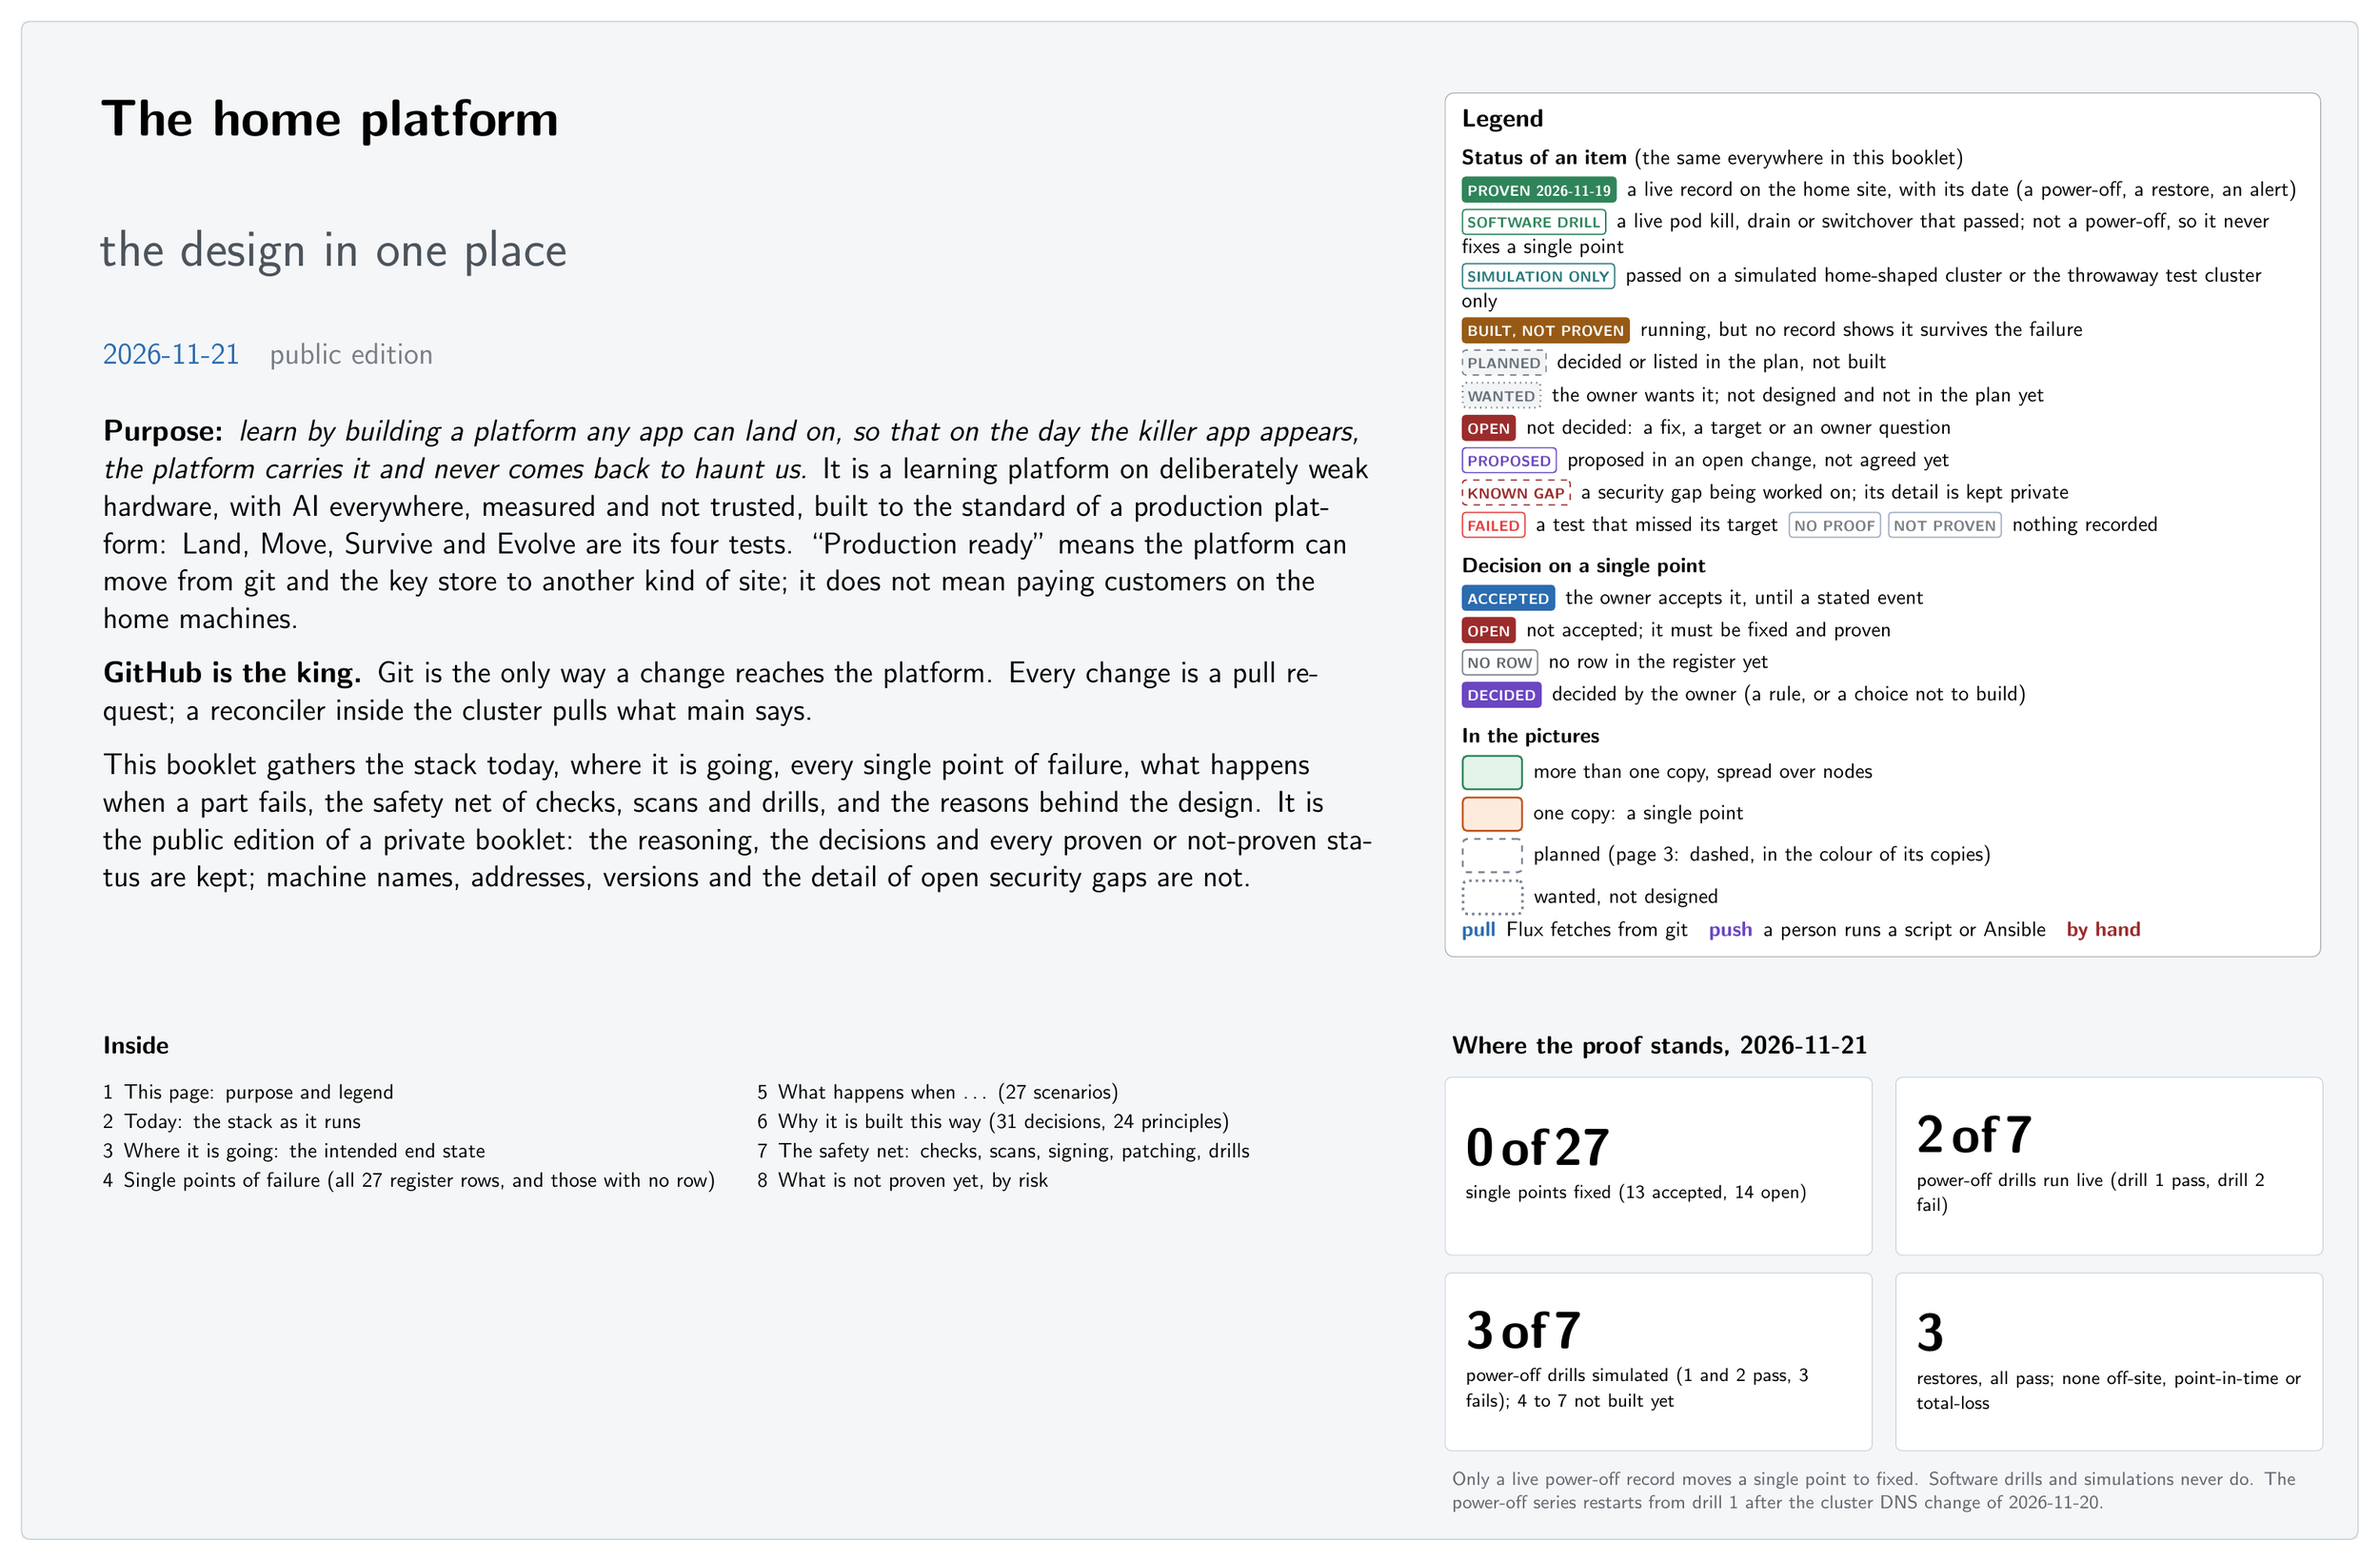
\begin{tikzpicture}[x=1cm,y=1cm]
  \fill[band] (0,0) rectangle (39.4,25.6);
  \draw[bandline, line width=0.6pt, rounded corners=4pt] (0,0) rectangle (39.4,25.6);
  \node[anchor=north west, font=\bfseries\fontsize{40}{46}\selectfont] at (1.2,24.4) {The home platform};
  \node[anchor=north west, font=\fontsize{28}{34}\selectfont, text=ink!80] at (1.2,22.2) {the design in one place};
  \node[anchor=north west, font=\Large, text=pull] at (1.25,20.3) {2026-11-21\quad\color{ink!60}public edition};
  \node[anchor=north west, text width=21.5cm, font=\Large, align=left] at (1.25,19.0) {%
    \textbf{Purpose:} \emph{learn by building a platform any app can land on, so that on the day the killer app appears,
    the platform carries it and never comes back to haunt us.} It is a learning platform on deliberately weak hardware, with AI
    everywhere, measured and not trusted, built to the standard of a production platform: Land, Move, Survive and Evolve are its
    four tests. ``Production ready'' means the platform can move from git and the key store to another kind of site; it does not
    mean paying customers on the home machines.\\[8pt]
    \textbf{GitHub is the king.} Git is the only way a change reaches the platform. Every change is a pull
    request; a reconciler inside the cluster pulls what main says.\\[8pt]
    This booklet gathers the stack today, where it is going, every single point of failure, what happens when a part fails, the safety net of checks, scans and drills,
    and the reasons behind the design. It is the public edition of a private booklet: the reasoning, the decisions and every
    proven or not-proven status are kept; machine names, addresses, versions and the detail of open security gaps are not.};

  % contents
  \node[anchor=north west, font=\bfseries\large] at (1.25,8.6) {Inside};
  \node[anchor=north west, text width=21cm, align=left] at (1.25,7.9) {%
    \begin{tabular}{@{}r@{\enspace}l@{\qquad}r@{\enspace}l@{}}
    1 & This page: purpose and legend & 5 & What happens when \dots\ (27 scenarios)\\
    2 & Today: the stack as it runs & 6 & Why it is built this way (31 decisions, 24 principles)\\
    3 & Where it is going: the intended end state & 7 & The safety net: checks, scans, signing, patching, drills\\
    4 & Single points of failure (all 27 register rows, and those with no row) & 8 & What is not proven yet, by risk\\
    \end{tabular}};

  % numbers strip
  \node[anchor=north west, font=\bfseries\large] at (24.0,8.6) {Where the proof stands, 2026-11-21};
  \foreach \x/\y/\bnum/\btxt in {24.0/7.8/0 of 27/{single points fixed (13 accepted, 14 open)},
                              31.6/7.8/2 of 7/{power-off drills run live (drill 1 pass, drill 2 fail)},
                              24.0/4.5/3 of 7/{power-off drills simulated (1 and 2 pass, 3 fails); 4 to 7 not built yet},
                              31.6/4.5/3/{restores, all pass; none off-site, point-in-time or total-loss}}{
    \node[anchor=north west, draw=bandline, fill=white, rounded corners=3pt, minimum width=7.2cm, minimum height=3.0cm,
          text width=6.5cm, align=left] at (\x,\y) {{\fontsize{26}{30}\selectfont\bfseries \bnum}\\[4pt]\small \btxt};}
  \node[anchor=north west, text width=15cm, font=\small, text=ink!70] at (24.0,1.25) {%
    Only a live power-off record moves a single point to fixed. Software drills and simulations never do. The power-off series
    restarts from drill 1 after the cluster DNS change of 2026-11-20.};

  % legend
  \node[anchor=north west, draw=ink!40, fill=white, rounded corners=4pt, text width=14.2cm, align=left, inner sep=8pt] at (24.0,24.4) {%
    {\large\bfseries Legend}\\[6pt]
    \textbf{Status of an item} (the same everywhere in this booklet)\\[3pt]
    \stProven[2026-11-19]\enspace a live record on the home site, with its date (a power-off, a restore, an alert)\\[2pt]
    \stDrill\enspace a live pod kill, drain or switchover that passed; not a power-off, so it never fixes a single point\\[2pt]
    \stSim\enspace passed on a simulated home-shaped cluster or the throwaway test cluster only\\[2pt]
    \stBuilt\enspace running, but no record shows it survives the failure\\[2pt]
    \stPlanned\enspace decided or listed in the plan, not built\\[2pt]
    \stWanted\enspace the owner wants it; not designed and not in the plan yet\\[2pt]
    \stOpen\enspace not decided: a fix, a target or an owner question\\[2pt]
    \stProp\enspace proposed in an open change, not agreed yet\\[2pt]
    \stGap\enspace a security gap being worked on; its detail is kept private\\[2pt]
    \stFailed\enspace a test that missed its target\enspace \stNone\ \stNotProven\enspace nothing recorded\\[8pt]
    \textbf{Decision on a single point}\\[3pt]
    \dAcc\enspace the owner accepts it, until a stated event\\[2pt]
    \dOpen\enspace not accepted; it must be fixed and proven\\[2pt]
    \dNoRow\enspace no row in the register yet\\[2pt]
    \dDecided\enspace decided by the owner (a rule, or a choice not to build)\\[8pt]
    \textbf{In the pictures}\\[3pt]
    \tikz[baseline={([yshift=-0.6ex]current bounding box.center)}]\node[draw=multi,fill=multifill,line width=0.9pt,rounded corners=2pt,minimum width=1cm,minimum height=0.42cm]{};\enspace more than one copy, spread over nodes\\[2pt]
    \tikz[baseline={([yshift=-0.6ex]current bounding box.center)}]\node[draw=single,fill=singlefill,line width=0.9pt,rounded corners=2pt,minimum width=1cm,minimum height=0.42cm]{};\enspace one copy: a single point\\[2pt]
    \tikz[baseline={([yshift=-0.6ex]current bounding box.center)}]\node[draw=plan,dashed,line width=0.9pt,rounded corners=2pt,minimum width=1cm,minimum height=0.42cm]{};\enspace planned (page 3: dashed, in the colour of its copies)\\[2pt]
    \tikz[baseline={([yshift=-0.6ex]current bounding box.center)}]\node[draw=plan,dotted,line width=1.2pt,rounded corners=2pt,minimum width=1cm,minimum height=0.42cm]{};\enspace wanted, not designed\\[2pt]
    \textcolor{pull}{\textbf{pull}}\enspace Flux fetches from git\quad
    \textcolor{push}{\textbf{push}}\enspace a person runs a script or Ansible\quad
    \textcolor{hand}{\textbf{by hand}}};
\end{tikzpicture}

% ================================================================== 2. TODAY
\Part{2}{Today: the stack as it runs}{The one-page stack picture of 2026-11-21, checked against the cluster and the private repository that day (the same picture as on the platform page).
Green means more than one copy runs, not that a power-off proved it.}
\begin{center}
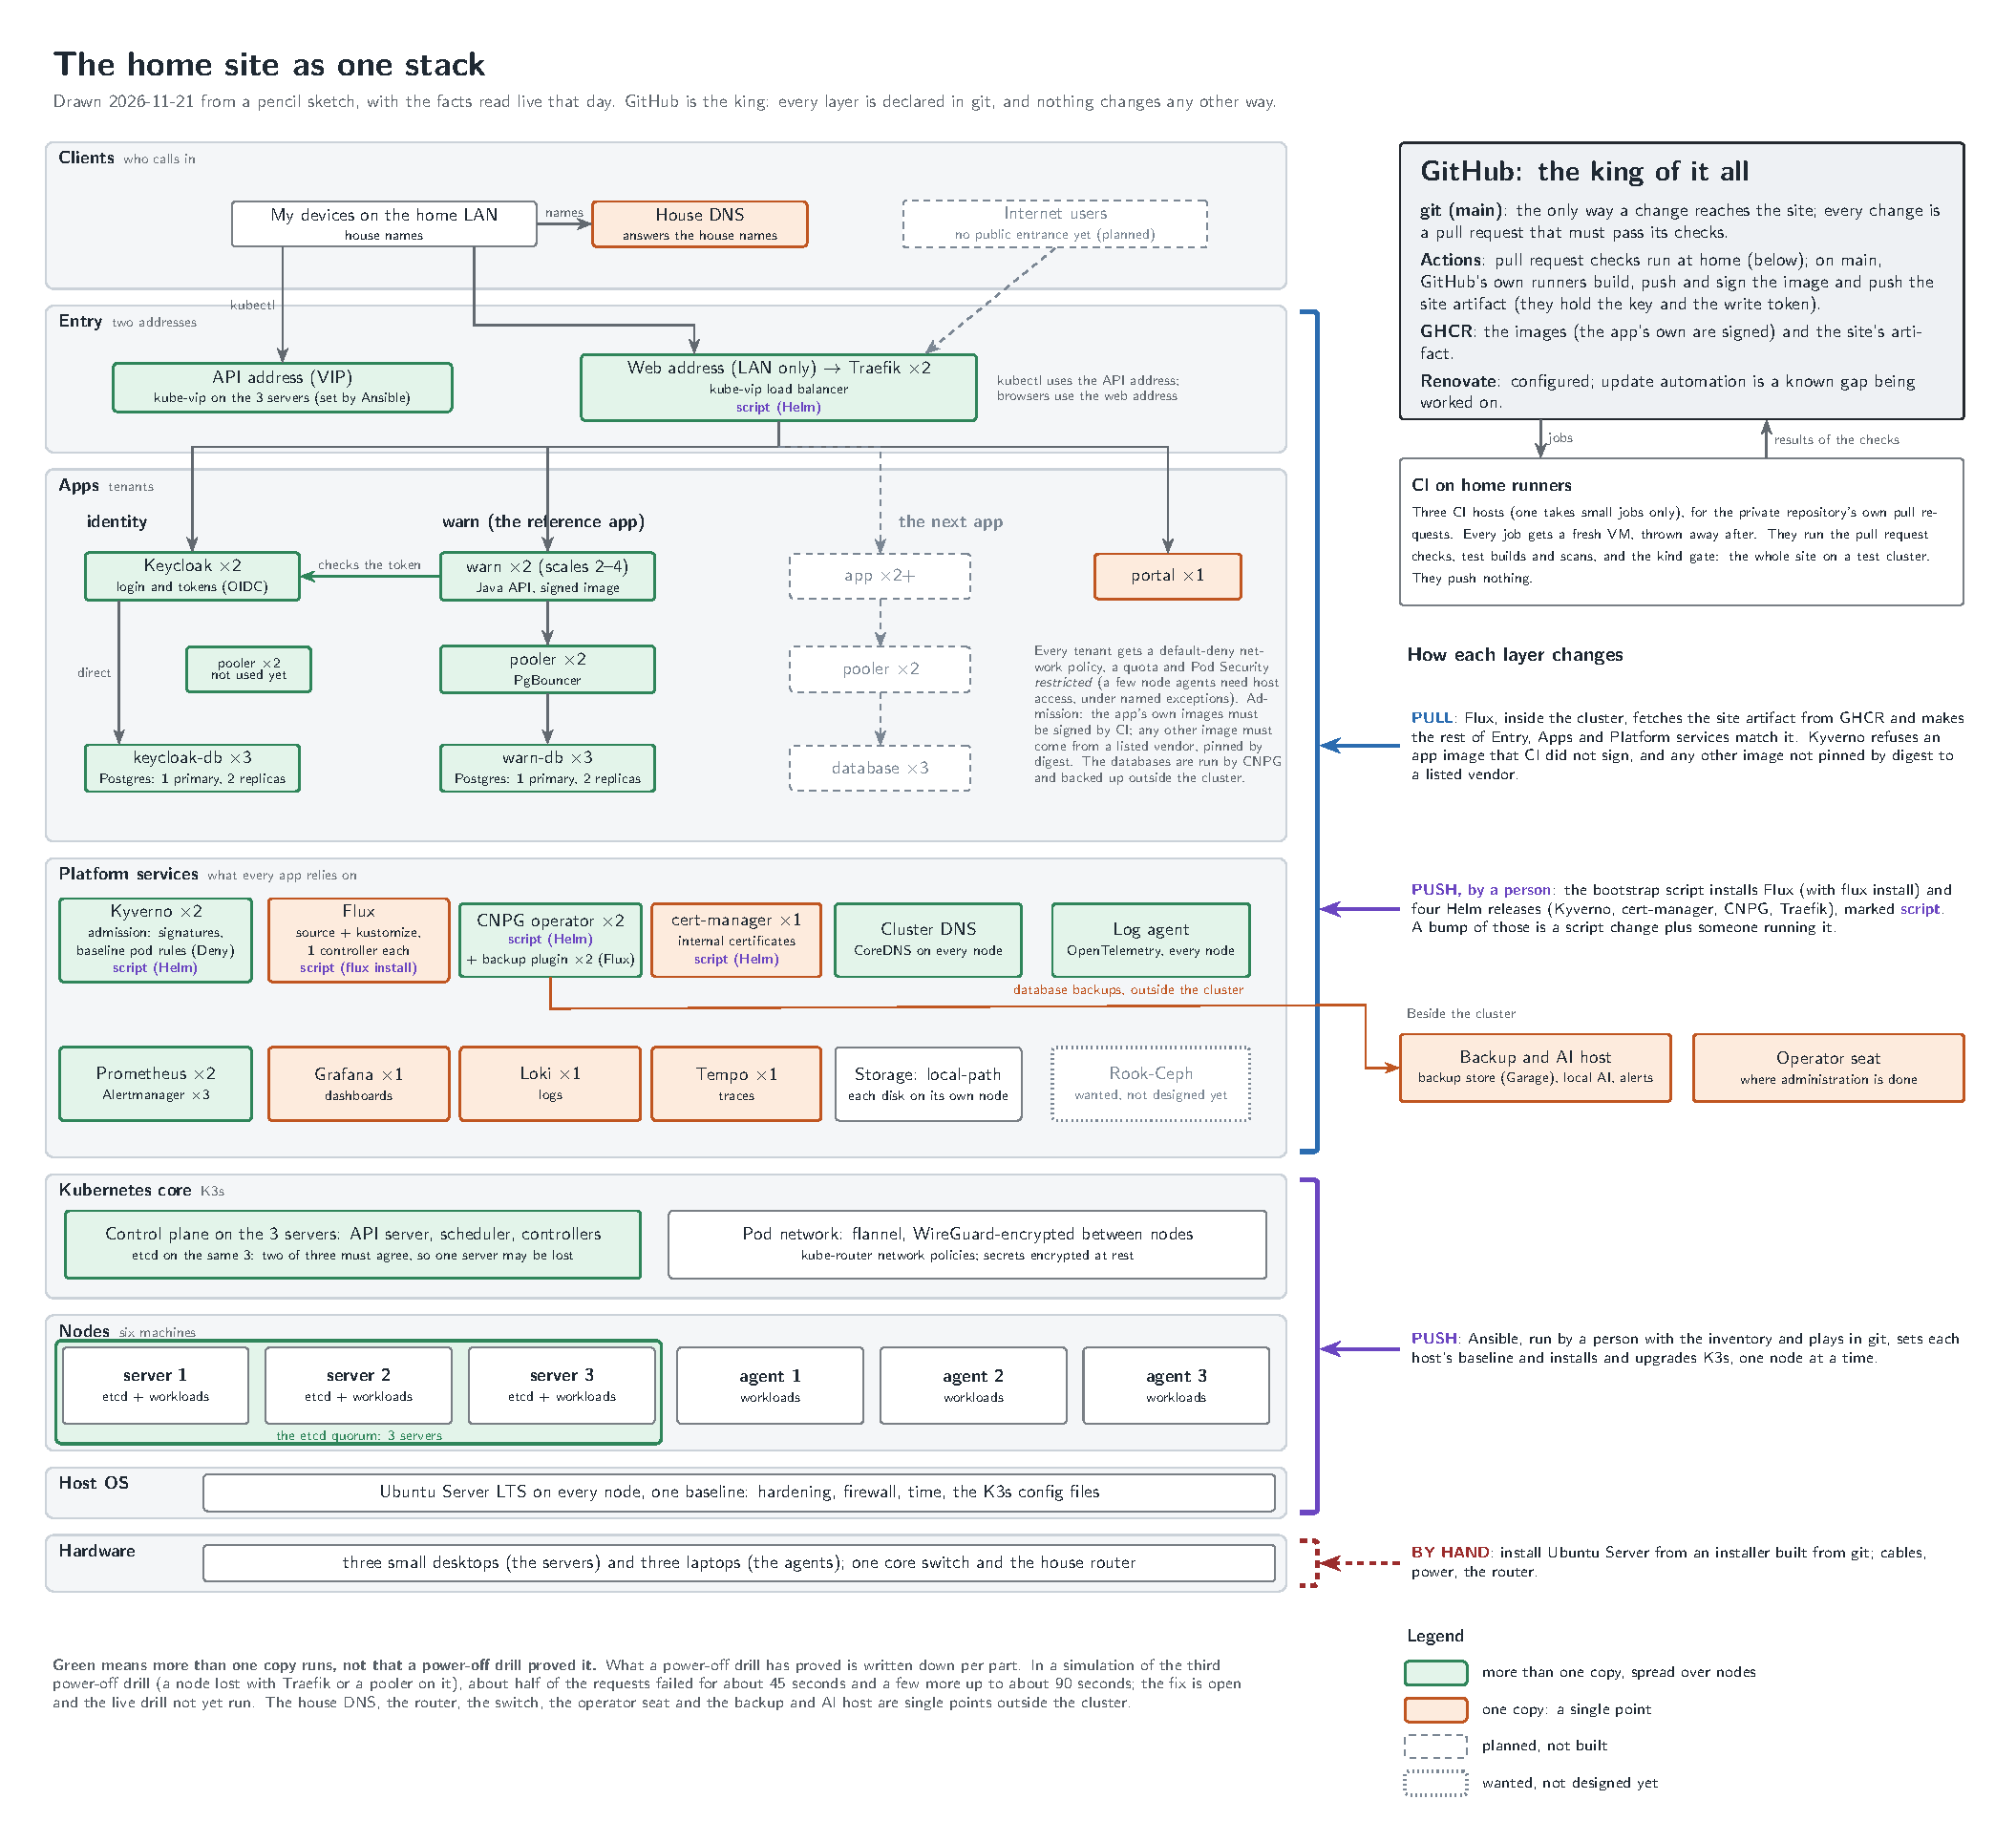
\includegraphics[width=\textwidth,height=0.9\textheight,keepaspectratio]{../diagrams/stack.pdf}
\end{center}

% ================================================================== 3. WHERE IT IS GOING
\Part{3}{Where it is going: the intended end state}{The same stack, drawn from the decisions and the plan. Fill = copies at the end. Outline: solid built, dashed planned (or only proposed, tagged so), dotted wanted.
The tag in each box gives its status. Orange boxes stay single at the end, or are undecided (tagged OPEN).}
\vspace{-2mm}
\begin{center}
\resizebox{!}{0.9\textheight}{%
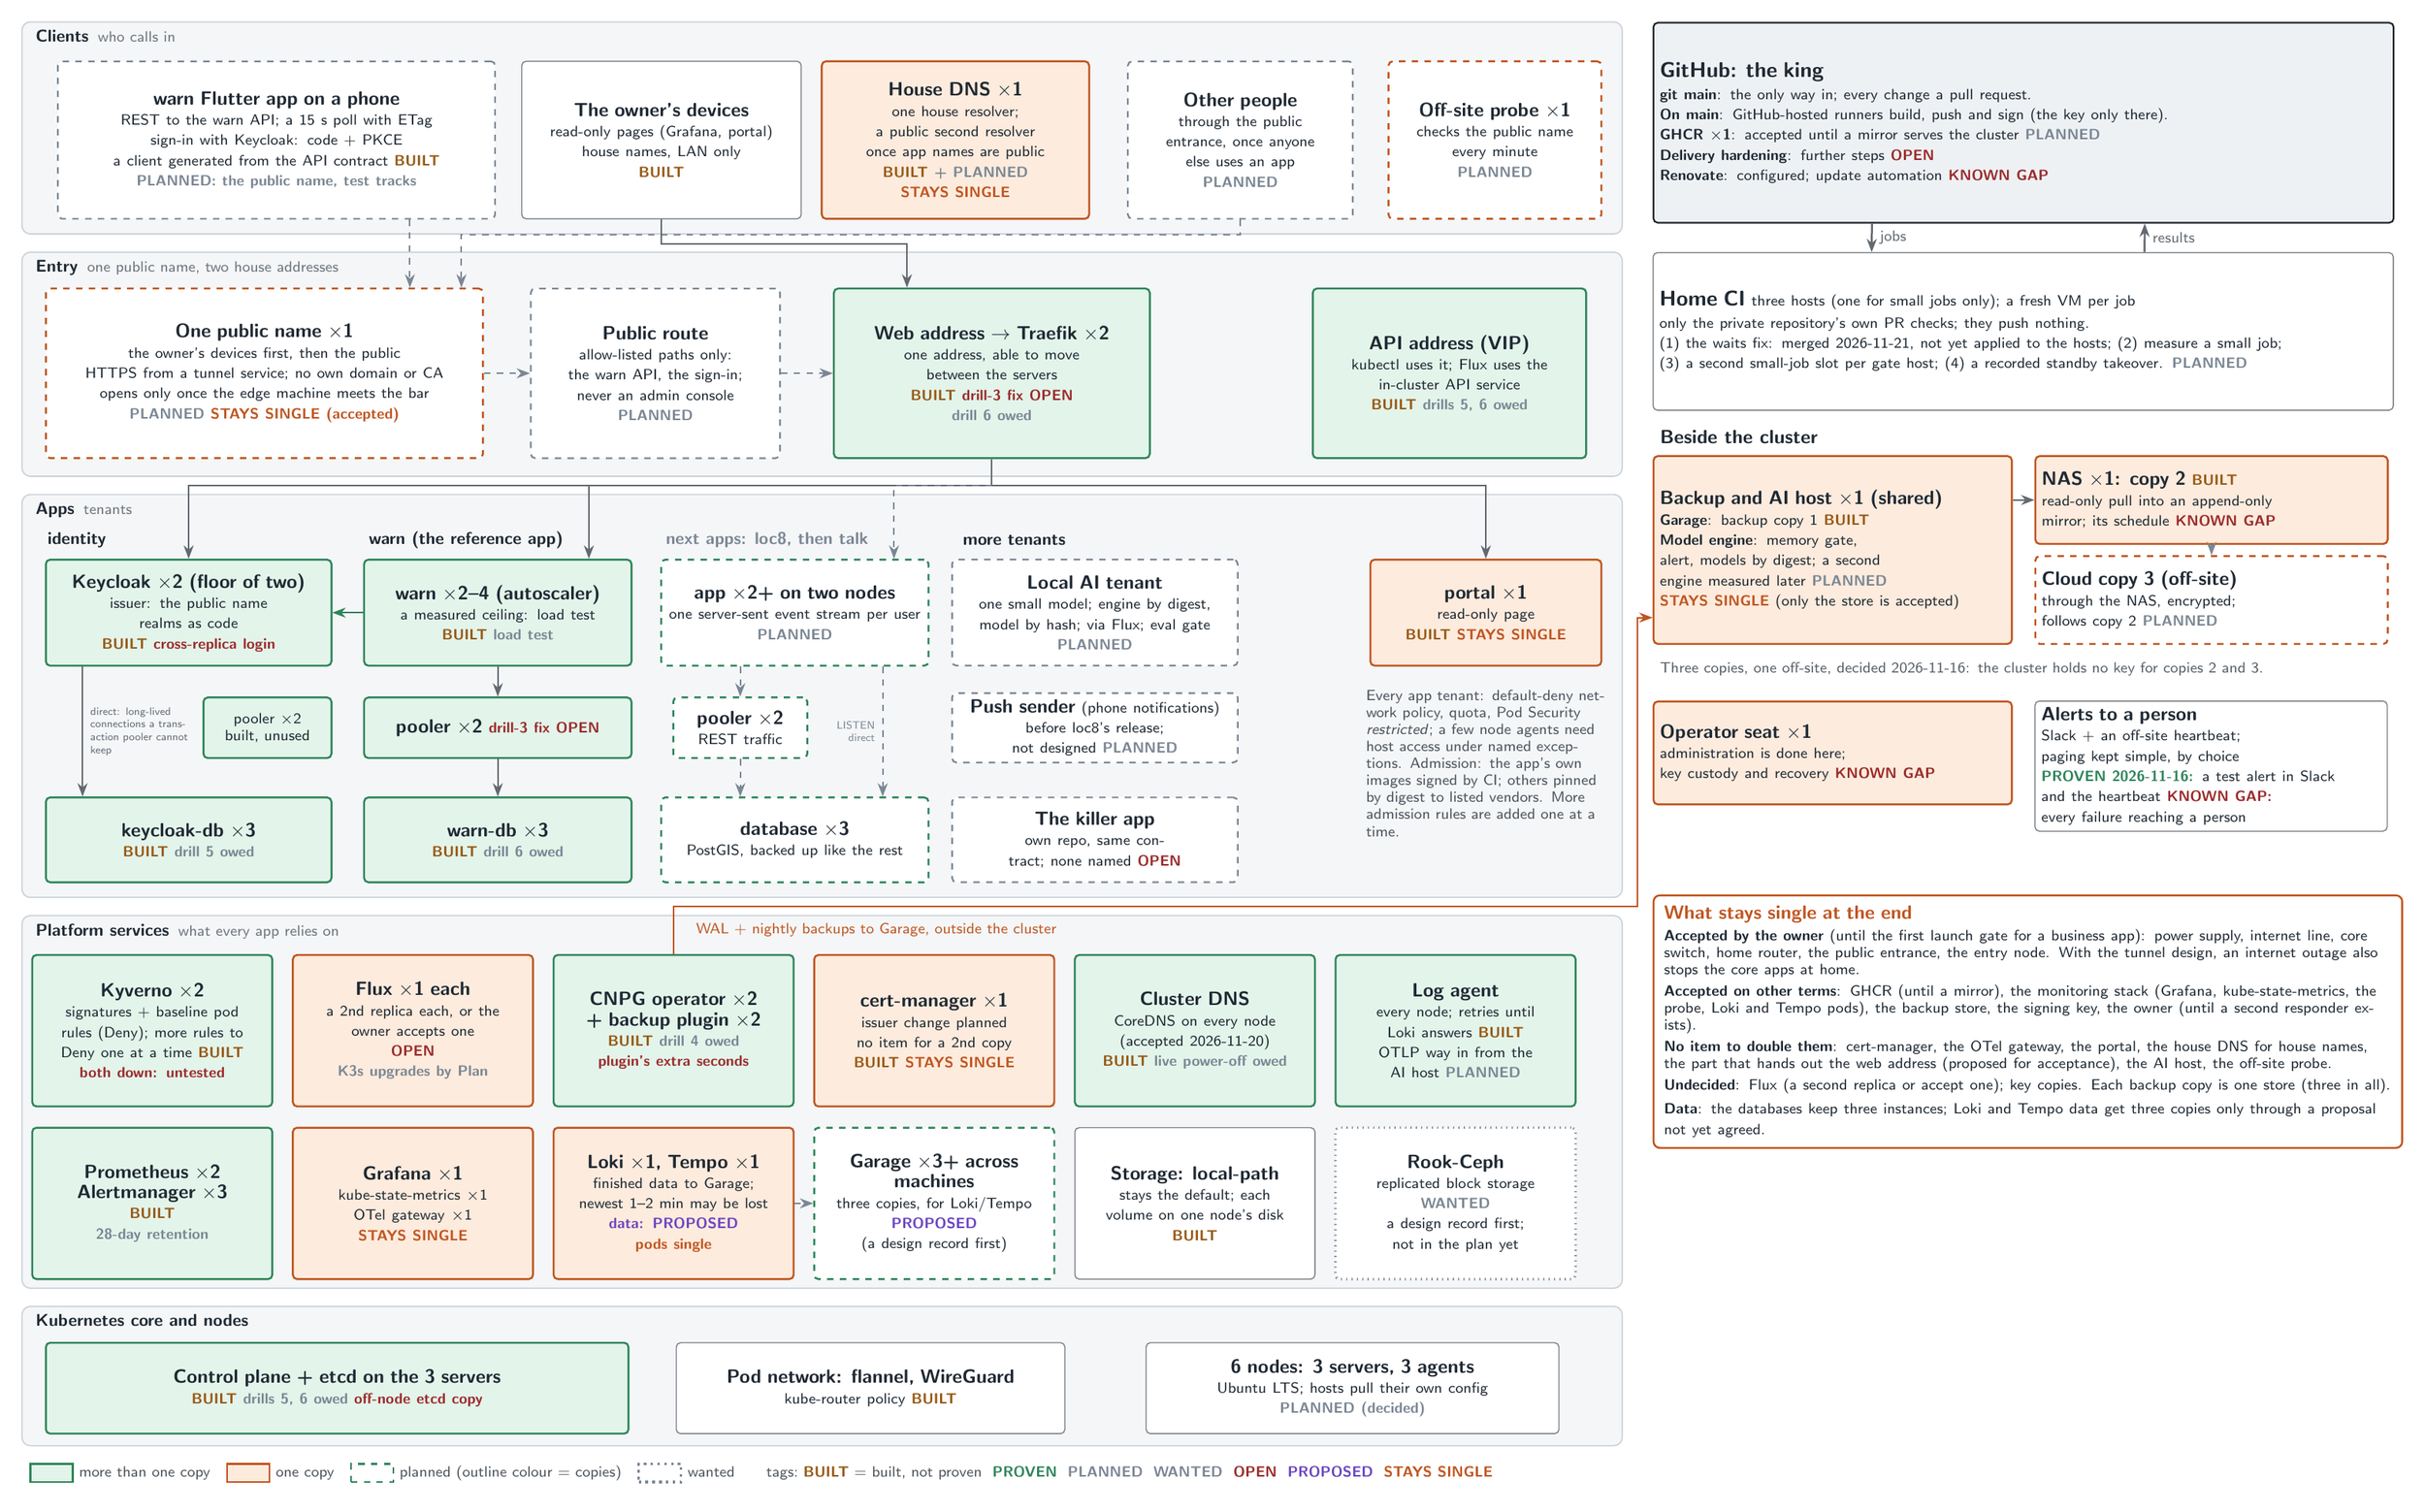
\begin{tikzpicture}[x=1cm, y=1cm,
  every node/.style={font=\footnotesize, text=ink},
  layer/.style={draw=bandline, fill=band, rounded corners=4pt, line width=0.6pt},
  box/.style={draw=ink!60, fill=white, rounded corners=2pt, align=center, inner sep=3pt, line width=0.5pt},
  multi/.style={box, draw=multi, fill=multifill, line width=0.9pt},
  single/.style={box, draw=single, fill=singlefill, line width=0.9pt},
  pmulti/.style={box, draw=multi, dashed, fill=white, line width=0.9pt},
  psingle/.style={box, draw=single, dashed, fill=white, line width=0.9pt},
  plan/.style={box, draw=plan, dashed, fill=white, line width=0.8pt},
  want/.style={box, draw=plan, dotted, fill=white, line width=1.2pt},
  ghbox/.style={box, draw=gh, fill=ghfill, line width=0.8pt},
  flow/.style={-{Stealth[length=2.2mm]}, line width=0.7pt, draw=ink!70},
  pflow/.style={flow, dashed, draw=plan},
  tag/.style={font=\scriptsize, text=ink!70},
]
\newcommand{\nm}[1]{{\small\bfseries #1}}
\newcommand{\tB}[1]{{\scriptsize\bfseries\color{builtc}#1}}
\newcommand{\tP}[1]{{\scriptsize\bfseries\color{plan}#1}}
\newcommand{\tW}[1]{{\scriptsize\bfseries\itshape\color{plan}#1}}
\newcommand{\tO}[1]{{\scriptsize\bfseries\color{hand}#1}}
\newcommand{\tS}[1]{{\scriptsize\bfseries\color{single}#1}}
\newcommand{\tG}[1]{{\scriptsize\bfseries\color{multi}#1}}
\newcommand{\tR}[1]{{\scriptsize\bfseries\color{push}#1}}
\newcommand{\ds}[1]{{\scriptsize #1}}

% ---------------------------------------------------------------- bands (x 0..26.4)
\newcommand{\band}[4]{%
  \draw[layer] (0,#1) rectangle (26.4,#2);
  \node[anchor=north west, inner sep=2pt] at (0.15,#2-0.06) {\textbf{#3}\enspace{\scriptsize\color{ink!65}#4}};}
\band{20.9}{24.4}{Clients}{who calls in}
\band{16.9}{20.6}{Entry}{one public name, two house addresses}
\band{9.95}{16.6}{Apps}{tenants}
\band{3.5}{9.65}{Platform services}{what every app relies on}
\band{0.9}{3.2}{Kubernetes core and nodes}{}

% ---------------------------------------------------------------- clients (boxes 21.15..23.85)
\node[plan, text width=7.0cm, minimum height=2.6cm] (phone) at (4.2,22.45) {%
  \nm{warn Flutter app on a phone}\\
  \ds{REST to the warn API; a 15 s poll with ETag}\\
  \ds{sign-in with Keycloak: code + PKCE}\\
  \ds{a client generated from the API contract} \tB{BUILT}\\
  \tP{PLANNED: the public name, test tracks}};
\node[box, text width=4.4cm, minimum height=2.6cm] (lan) at (10.55,22.45) {%
  \nm{The owner's devices}\\ \ds{read-only pages (Grafana, portal)}\\ \ds{house names, LAN only}\\ \tB{BUILT}};
\node[single, text width=4.2cm, minimum height=2.6cm] (hdns) at (15.4,22.45) {%
  \nm{House DNS \X1}\\ \ds{one house resolver;}\\ \ds{a public second resolver}\\ \ds{once app names are public}\\
  \tB{BUILT}\ \tP{+ PLANNED}\\ \tS{STAYS SINGLE}};
\node[plan, text width=3.5cm, minimum height=2.6cm] (others) at (20.1,22.45) {%
  \nm{Other people}\\ \ds{through the public}\\ \ds{entrance, once anyone}\\ \ds{else uses an app}\\ \tP{PLANNED}};
\node[psingle, text width=3.3cm, minimum height=2.6cm] (probe) at (24.3,22.45) {%
  \nm{Off-site probe \X1}\\ \ds{checks the public name}\\ \ds{every minute}\\ \tP{PLANNED}};

% ---------------------------------------------------------------- entry (boxes 17.15..20.05)
\node[psingle, text width=7.0cm, minimum height=2.8cm] (edge) at (4.0,18.6) {%
  \nm{One public name \X1}\\
  \ds{the owner's devices first, then the public}\\
  \ds{HTTPS from a tunnel service; no own domain or CA}\\
  \ds{opens only once the edge machine meets the bar}\\
  \tP{PLANNED}\ \tS{STAYS SINGLE (accepted)}};
\node[plan, text width=3.9cm, minimum height=2.8cm] (route) at (10.45,18.6) {%
  \nm{Public route}\\ \ds{allow-listed paths only:}\\ \ds{the warn API, the sign-in;}\\ \ds{never an admin console}\\ \tP{PLANNED}};
\node[multi, text width=5.0cm, minimum height=2.8cm] (web) at (16.0,18.6) {%
  \nm{Web address \ensuremath{\to} Traefik \X2}\\ \ds{one address, able to move}\\ \ds{between the servers}\\
  \tB{BUILT}\ \tO{drill-3 fix OPEN}\\ \tP{drill 6 owed}};
\node[multi, text width=4.3cm, minimum height=2.8cm] (api) at (23.55,18.6) {%
  \nm{API address (VIP)}\\ \ds{kubectl uses it; Flux uses the}\\ \ds{in-cluster API service}\\ \tB{BUILT}\ \tP{drills 5, 6 owed}};
\draw[pflow] ($(phone.south)+(2.2,0)$) -- ($(edge.north)+(2.4,0)$);
\draw[pflow] (others.south) -- ++(0,-0.25) -| ($(edge.north)+(3.25,0)$);
\draw[pflow] (edge.east) -- (route.west);
\draw[pflow] (route.east) -- (web.west);
\draw[flow] (lan.south) -- ++(0,-0.4) -| ($(web.north)+(-1.4,0)$);

% ---------------------------------------------------------------- apps
\node[font=\bfseries\footnotesize, anchor=west] at (0.3,15.85) {identity};
\node[multi, text width=4.5cm, minimum height=1.75cm] (kc) at (2.75,14.65) {%
  \nm{Keycloak \X2 (floor of two)}\\ \ds{issuer: the public name}\\ \ds{realms as code}\\
  \tB{BUILT}\ \tO{cross-replica login}};
\node[multi, text width=1.9cm, minimum height=1.0cm, font=\scriptsize] (kcpool) at (4.05,12.75) {pooler \X2\\ built, unused};
\node[multi, text width=4.5cm, minimum height=1.4cm] (kcdb) at (2.75,10.9) {%
  \nm{keycloak-db \X3}\\ \tB{BUILT}\ \tP{drill 5 owed}};
\draw[flow] ($(kc.south)+(-1.75,0)$) -- node[right, tag, align=left, text width=1.7cm, font=\tiny] {direct: long-lived connections a transaction pooler cannot keep} ($(kcdb.north)+(-1.75,0)$);

\node[font=\bfseries\footnotesize, anchor=west] (warnlbl) at (5.6,15.85) {warn (the reference app)};
\node[multi, text width=4.2cm, minimum height=1.75cm] (warn) at (7.85,14.65) {%
  \nm{warn \X2--4 (autoscaler)}\\ \ds{a measured ceiling: load test}\\ \tB{BUILT}\ \tP{load test}};
\node[multi, text width=4.2cm, minimum height=1.0cm] (wpool) at (7.85,12.75) {\nm{pooler \X2}\ \tO{drill-3 fix OPEN}};
\node[multi, text width=4.2cm, minimum height=1.4cm] (wdb) at (7.85,10.9) {\nm{warn-db \X3}\\ \tB{BUILT}\ \tP{drill 6 owed}};
\draw[flow] (warn) -- (wpool);
\draw[flow] (wpool) -- (wdb);
\draw[flow, draw=multi] (warn.west) -- (kc.east);

\node[font=\bfseries\footnotesize, anchor=west, text=plan] (xapplbl) at (10.5,15.85) {next apps: loc8, then talk};
\node[pmulti, text width=4.2cm, minimum height=1.75cm] (xapp) at (12.75,14.65) {%
  \nm{app \X2+ on two nodes}\\ \ds{one server-sent event stream per user}\\ \tP{PLANNED}};
\node[pmulti, text width=2.0cm, minimum height=1.0cm] (xpool) at (11.85,12.75) {\nm{pooler \X2}\\ \ds{REST traffic}};
\node[pmulti, text width=4.2cm, minimum height=1.4cm] (xdb) at (12.75,10.9) {\nm{database \X3}\\ \ds{PostGIS, backed up like the rest}};
\draw[pflow] (xpool.north |- xapp.south) -- (xpool.north);
\draw[pflow] (xpool.south) -- (xpool.south |- xdb.north);
\draw[pflow] ($(xapp.south)+(1.45,0)$) -- node[left, tag, align=right, text=plan, font=\tiny] {LISTEN\\direct} ($(xdb.north)+(1.45,0)$);

\node[font=\bfseries\footnotesize, anchor=west] at (15.4,15.85) {more tenants};
\node[plan, text width=4.5cm, minimum height=1.75cm] (ai) at (17.7,14.65) {%
  \nm{Local AI tenant}\\ \ds{one small model; engine by digest,}\\ \ds{model by hash; via Flux; eval gate}\\ \tP{PLANNED}};
\node[plan, text width=4.5cm, minimum height=1.0cm] (pushs) at (17.7,12.75) {%
  \nm{Push sender} \ds{(phone notifications)}\\ \ds{before loc8's release; not designed} \tP{PLANNED}};
\node[plan, text width=4.5cm, minimum height=1.4cm] (killer) at (17.7,10.9) {%
  \nm{The killer app}\\ \ds{own repo, same contract; none named} \tO{OPEN}};

\node[single, text width=3.6cm, minimum height=1.75cm] (portal) at (24.15,14.65) {%
  \nm{portal \X1}\\ \ds{read-only page}\\ \tB{BUILT}\ \tS{STAYS SINGLE}};
\node[anchor=north west, text width=4.0cm, font=\scriptsize, text=ink!80, align=left] at (22.05,13.5) {%
  Every app tenant: default-deny network policy, quota, Pod Security \emph{restricted}; a few node agents need host access under named exceptions. Admission: the app's own images signed by CI;
  others pinned by digest to listed vendors. More admission rules are added one at a time.};

% web address fan into the apps
\coordinate (fan) at (16.0,16.75);
\draw[line width=0.7pt, draw=ink!70] (web.south) -- (fan);
\draw[flow] (fan) -| (kc.north);
\draw[flow] (fan) -| ($(warnlbl.east)+(0.3,0)$) -- ($(warnlbl.east |- warn.north)+(0.3,0)$);
\draw[pflow] (fan) -| ($(xapplbl.east)+(0.3,0)$) -- ($(xapplbl.east |- xapp.north)+(0.3,0)$);
\draw[flow] (fan) -| (portal.north);

% ---------------------------------------------------------------- platform services
\newcommand{\svc}[5]{\node[#1, text width=#2, minimum height=2.5cm] (#3) at #4 {#5};}
\svc{multi}{3.75cm}{kyv}{(2.15,7.75)}{\nm{Kyverno \X2}\\ \ds{signatures + baseline pod}\\ \ds{rules (Deny); more rules to}\\ \ds{Deny one at a time} \tB{BUILT}\\ \tO{both down: untested}}
\svc{single}{3.75cm}{flux}{(6.45,7.75)}{\nm{Flux \X1 each}\\ \ds{a 2nd replica each, or the}\\ \ds{owner accepts one}\\ \tO{OPEN}\\ \tP{K3s upgrades by Plan}}
\svc{multi}{3.75cm}{cnpg}{(10.75,7.75)}{\nm{CNPG operator \X2}\\ \nm{+ backup plugin \X2}\\ \tB{BUILT}\ \tP{drill 4 owed}\\ \tO{plugin's extra seconds}}
\svc{single}{3.75cm}{certm}{(15.05,7.75)}{\nm{cert-manager \X1}\\ \ds{issuer change planned}\\ \ds{no item for a 2nd copy}\\ \tB{BUILT}\ \tS{STAYS SINGLE}}
\svc{multi}{3.75cm}{dns}{(19.35,7.75)}{\nm{Cluster DNS}\\ \ds{CoreDNS on every node}\\ \ds{(accepted 2026-11-20)}\\ \tB{BUILT}\ \tP{live power-off owed}}
\svc{multi}{3.75cm}{logag}{(23.65,7.75)}{\nm{Log agent}\\ \ds{every node; retries until}\\ \ds{Loki answers} \tB{BUILT}\\ \ds{OTLP way in from the}\\ \ds{AI host} \tP{PLANNED}}

\svc{multi}{3.75cm}{prom}{(2.15,4.9)}{\nm{Prometheus \X2}\\ \nm{Alertmanager \X3}\\ \tB{BUILT}\\ \tP{28-day retention}}
\svc{single}{3.75cm}{graf}{(6.45,4.9)}{\nm{Grafana \X1}\\ \ds{kube-state-metrics \X1}\\ \ds{OTel gateway \X1}\\ \tS{STAYS SINGLE}}
\svc{single}{3.75cm}{loki}{(10.75,4.9)}{\nm{Loki \X1, Tempo \X1}\\ \ds{finished data to Garage;}\\ \ds{newest 1--2 min may be lost}\\ \tR{data: PROPOSED}\\ \tS{pods single}}
\svc{pmulti}{3.75cm}{garc}{(15.05,4.9)}{\nm{Garage \X3+ across}\\ \nm{machines}\\ \ds{three copies, for Loki/Tempo}\\ \tR{PROPOSED}\\ \ds{(a design record first)}}
\svc{box}{3.75cm}{lp}{(19.35,4.9)}{\nm{Storage: local-path}\\ \ds{stays the default; each}\\ \ds{volume on one node's disk}\\ \tB{BUILT}}
\svc{want}{3.75cm}{ceph}{(23.65,4.9)}{\nm{Rook-Ceph}\\ \ds{replicated block storage}\\ \tW{WANTED}\\ \ds{a design record first;}\\ \ds{not in the plan yet}}
\draw[pflow] (loki.east) -- (garc.west);

% ---------------------------------------------------------------- core and nodes (boxes 1.1..2.6)
\node[multi, text width=9.4cm, minimum height=1.5cm] (cp) at (5.2,1.85) {%
  \nm{Control plane + etcd on the 3 servers}\\ \tB{BUILT}\ \tP{drills 5, 6 owed}\ \tO{off-node etcd copy}};
\node[box, text width=6.2cm, minimum height=1.5cm] (pnet) at (14.0,1.85) {%
  \nm{Pod network: flannel, WireGuard}\\ \ds{kube-router policy}\ \tB{BUILT}};
\node[box, text width=6.6cm, minimum height=1.5cm] (nodes) at (21.95,1.85) {%
  \nm{6 nodes: 3 servers, 3 agents}\\ \ds{Ubuntu LTS; hosts pull their own config}\\ \tP{PLANNED (decided)}};

% ================================================================ right column (x 26.9..39.3)
\node[ghbox, text width=12.0cm, minimum height=3.3cm, align=left, anchor=north west] (gh) at (26.9,24.4) {%
  {\normalsize\bfseries GitHub: the king}\\[1pt]
  \ds{\textbf{git main}: the only way in; every change a pull request.}\\
  \ds{\textbf{On main}: GitHub-hosted runners build, push and sign (the key only there).}\\
  \ds{\textbf{GHCR \X1}: accepted until a mirror serves the cluster} \tP{PLANNED}\\
  \ds{\textbf{Delivery hardening}: further steps} \tO{OPEN}\\
  \ds{\textbf{Renovate}: configured; update automation} \tO{KNOWN GAP}};
\node[box, text width=12.0cm, minimum height=2.6cm, align=left, anchor=north west] (ci) at (26.9,20.6) {%
  {\normalsize\bfseries Home CI}\ \ds{three hosts (one for small jobs only); a fresh VM per job}\\[1pt]
  \ds{only the private repository's own PR checks; they push nothing.}\\
  \ds{(1) the waits fix: merged 2026-11-21, not yet applied to the hosts; (2) measure a small job;}\\
  \ds{(3) a second small-job slot per gate host; (4) a recorded standby takeover.}\enspace \tP{PLANNED}};
\draw[flow, line width=0.9pt] ($(gh.south)+(-2.5,0)$) -- node[right, tag] {jobs} ($(ci.north)+(-2.5,0)$);
\draw[flow, line width=0.9pt] ($(ci.north)+(2.0,0)$) -- node[right, tag] {results} ($(gh.south)+(2.0,0)$);

\node[anchor=west, font=\bfseries\small] at (26.9,17.55) {Beside the cluster};
\node[single, text width=5.7cm, minimum height=3.1cm, align=left, anchor=north west] (mini) at (26.9,17.25) {%
  \nm{Backup and AI host \X1 (shared)}\\
  \ds{\textbf{Garage}: backup copy 1} \tB{BUILT}\\
  \ds{\textbf{Model engine}: memory gate,}\\ \ds{alert, models by digest; a second}\\ \ds{engine measured later} \tP{PLANNED}\\
  \tS{STAYS SINGLE}\ \ds{(only the store is accepted)}};
\node[single, text width=5.6cm, minimum height=1.45cm, align=left, anchor=north west] (nas) at (33.2,17.25) {%
  \nm{NAS \X1: copy 2}\ \tB{BUILT}\\ \ds{read-only pull into an append-only}\\ \ds{mirror; its schedule} \tO{KNOWN GAP}};
\node[psingle, text width=5.6cm, minimum height=1.45cm, align=left, anchor=north west] (cloud) at (33.2,15.6) {%
  \nm{Cloud copy 3 (off-site)}\\ \ds{through the NAS, encrypted;}\\ \ds{follows copy 2} \tP{PLANNED}};
\draw[flow] (mini.east |- nas.west) -- (nas.west);
\draw[pflow] (nas.south) -- (cloud.north);
\draw[flow, draw=single] (cnpg.north) -- (10.75,9.8) -- (26.65,9.8) |- ($(mini.south west)+(0,0.45)$);
\node[tag, text=single, anchor=south west] at (11.0,9.18) {WAL + nightly backups to Garage, outside the cluster};
\node[anchor=north west, text width=12cm, font=\scriptsize, text=ink!75] at (26.9,13.95) {%
  Three copies, one off-site, decided 2026-11-16: the cluster holds no key for copies 2 and 3.};

\node[single, text width=5.7cm, minimum height=1.7cm, align=left, anchor=north west] (studio) at (26.9,13.2) {%
  \nm{Operator seat \X1}\\ \ds{administration is done here;}\\ \ds{key custody and recovery} \tO{KNOWN GAP}};
\node[box, text width=5.6cm, minimum height=1.7cm, align=left, anchor=north west] (alerts) at (33.2,13.2) {%
  \nm{Alerts to a person}\\ \ds{Slack + an off-site heartbeat;}\\ \ds{paging kept simple, by choice}\\ \tG{PROVEN 2026-11-16:} \ds{a test alert in Slack}\\ \ds{and the heartbeat} \tO{KNOWN GAP:}\\ \ds{every failure reaching a person}};

% stays single at the end
\node[draw=single, line width=0.9pt, fill=white, rounded corners=3pt, text width=12.0cm, align=left, anchor=north west, inner sep=5pt] (stay) at (26.9,10.0) {%
  {\small\bfseries\color{single} What stays single at the end}\\[2pt]
  \scriptsize
  \textbf{Accepted by the owner} (until the first launch gate for a business app): power supply, internet line, core switch,
  home router, the public entrance, the entry node. With the tunnel design, an internet outage also stops the core apps at home.\\[2pt]
  \textbf{Accepted on other terms}: GHCR (until a mirror), the monitoring stack (Grafana, kube-state-metrics, the probe, Loki and
  Tempo pods), the backup store, the signing key, the owner (until a second responder exists).\\[2pt]
  \textbf{No item to double them}: cert-manager, the OTel gateway, the portal, the house DNS for house names, the part that
  hands out the web address (proposed for acceptance), the AI host, the off-site probe.\\[2pt]
  \textbf{Undecided}: Flux (a second replica or accept one); key copies. Each backup copy is one store (three in all).\\[2pt]
  \textbf{Data}: the databases keep three instances; Loki and Tempo data get three copies only through a proposal not yet agreed.};

% legend strip
\node[anchor=west, font=\scriptsize, text=ink!80] at (0,0.45) {%
  \tikz[baseline={([yshift=-0.6ex]current bounding box.center)}]\node[draw=multi,fill=multifill,line width=0.9pt,minimum width=0.7cm,minimum height=0.3cm]{};\ more than one copy\quad
  \tikz[baseline={([yshift=-0.6ex]current bounding box.center)}]\node[draw=single,fill=singlefill,line width=0.9pt,minimum width=0.7cm,minimum height=0.3cm]{};\ one copy\quad
  \tikz[baseline={([yshift=-0.6ex]current bounding box.center)}]\node[draw=multi,dashed,line width=0.9pt,minimum width=0.7cm,minimum height=0.3cm]{};\ planned (outline colour = copies)\quad
  \tikz[baseline={([yshift=-0.6ex]current bounding box.center)}]\node[draw=plan,dotted,line width=1.2pt,minimum width=0.7cm,minimum height=0.3cm]{};\ wanted\qquad
  tags:\ \tB{BUILT} = built, not proven\ \ \tG{PROVEN}\ \ \tP{PLANNED}\ \ \tW{WANTED}\ \ \tO{OPEN}\ \ \tR{PROPOSED}\ \ \tS{STAYS SINGLE}};
\end{tikzpicture}}
\end{center}

% ================================================================== 4. SINGLE POINTS
\Part{4}{Single points of failure}{Every row of the single-points register (27: 13 accepted, 14 open, 0 fixed, every one with proof ``none'' in the register),
grouped by layer, plus the one-copy parts the register lacks (marked \dNoRow\ or \stProp). The proof column lists records outside the register: they never move a row to fixed. A software drill (pod kill, drain, switchover) carries the light green pill.}
{\footnotesize
\begin{longtable}{@{}L{5.3cm}L{3.3cm}L{7.5cm}L{7.9cm}L{7.3cm}L{6.6cm}@{}}
\textbf{What} & \textbf{Decision} & \textbf{Why, and what stops} & \textbf{Today} & \textbf{Target} & \textbf{Proof}\\\hline
\endfirsthead
\textbf{What} & \textbf{Decision} & \textbf{Why, and what stops} & \textbf{Today} & \textbf{Target} & \textbf{Proof}\\\hline
\endhead
\Group{6}{The site: power, network and names}
\textbf{Power supply}: one mains supply for the whole site & \dAcc\ 2026-11-08, until the first launch gate for a business app &
The owner's statement of 2026-11-08. Stops everything; a cold start follows. Left out of the availability budget. &
No UPS or second supply. No scripted shutdown and no wake-on-LAN yet. &
\stPlanned\ recovery side only: a scripted shutdown and start of the six nodes back to green. A second supply is not planned. &
\stNone\ The mains cut is not in the drill session.\\
\textbf{Internet line}: one provider, one line & \dAcc\ 2026-11-08, same terms &
Stops everything from outside and every outside service the apps call. With the tunnel design an outage also stops the core apps inside the house. &
No fix. & No fix planned. The tunnel design is revisited if the outage at home costs more than it saves. & \stNone\\
\textbf{Core switch}: one switch carries every server, storage and database host & \dAcc\ 2026-11-08, same terms &
A second switch helps only if every node has two network ports; most do not. Stops quorum, storage and every database together. &
No spare. & \stOpen\ a shelf spare is not decided. The proposed no-data-loss rule leaves the switch out. \stGap\ network segmentation. & \stNone\\
\textbf{Home router}: one router for the network and its names & \dAcc\ 2026-11-08, same terms &
Same reason as the switch. Stops the way in and out, and lookups that go through it. &
No spare. &
\stOpen\ shelf spare not decided. \stGap\ a record of its settings. & \stNone\\
\textbf{House DNS}: one resolver handed out by the router; the house names exist only there & \dOpen\ (accepted or open: an owner question) &
Stops lookups for every house device; phones lose warn and sign-in by name. Apps inside the cluster are not touched. &
\stBuilt\ one resolver. Settings read and recorded (2026-11-16). No backup or restore, no stop test. &
\stPlanned\ a public second resolver, handed out once the app names resolve publicly. Core apps move to one public name. &
\stNone\\
\Group{6}{Edge and entry}
\textbf{Public entrance}: one tunnel entrance on a small edge machine for every app & \dAcc\ 2026-11-08, until the first launch gate &
Stops every app from outside; the apps keep running. Left out of the availability budget. &
Not open: no app is published yet. It opens only after the edge machine and outside testing meet the platform's bar. &
\stPlanned\ one public name: the owner's devices first, the public when anyone else uses the app. Stays single by design. &
\stNone\\
\textbf{Entry node}: one node takes the traffic in from the entrance & \dAcc\ 2026-11-08 &
Stops the same as the entrance, until the address moves. Wording open: the address holder or a fixed node. &
The web address sits on one server at a time (read live 2026-11-21; it moved since the register's read of 2026-11-18). &
\stOpen\ reword the row; drill 6 reads it. & \stNone\\
\textbf{Service address}: the web address, able to move between the servers; one part (\X1) hands it out & \dOpen\ (the hand-out part \X1 is proposed for acceptance) &
Fixed when the holder is powered off and warn and the login realm answer on the same address within 30 s. The hand-out part stops only new addresses. &
\stBuilt\ on all three servers. &
\stPlanned\ drill 6; a simulation first (a simulation cannot prove address takeover on a real network). & \stNone\\
\textbf{Ingress}: Traefik \X2, disruption budget 1, spread only a preference & \dOpen &
Every app's way in. Fixed when one replica's node is powered off with the ingress still answering. Both replicas may land on one node. &
\stBuilt\ 2/2 on two nodes. In the simulated drill 3 about half of new connections failed until the node was NotReady: 175 of 9533 requests; back after 46--91 s against 30 s. &
\stOpen\ fix not chosen: shorter node-monitor grace, clients that retry a failed connect, a shorter connection-tracking timeout, or new targets. Simulated first. &
\stDrill[2026-11-16] pod kill 567/567.\ \stFailed[in simulation 2026-11-20] drill 3. Live drill 3 not run.\\
\Group{6}{Cluster core}
\textbf{Control plane}: API and etcd on three K3s servers; clients reach the API through one address that can move between the servers & \dOpen &
Address gone: kubectl and outside probes lose the API (Flux uses the in-cluster service). Two servers gone: nothing can change; running pods keep running. &
\stBuilt\ 3 servers Ready, upgraded one minor on 2026-11-18. &
\stPlanned\ drills 5 (API address holder) and 6 (etcd leader), each simulated first. &
\stSim[2026-11-11] test-cluster drain, 30/30 API probes. Live power-off owed.\\
\textbf{Cluster DNS}: CoreDNS on every node since 2026-11-20, same node first & \dOpen &
Live drill 2 (old two-replica design) stalled lookups on other nodes 51 s and failed two inserts. Fixed when a node with a DNS pod is off and no lookup elsewhere takes over 1 s. &
\stBuilt\ 6/6. Change-over with no failed lookup in 172,521 lookups; 2 fast failures in an earlier step unexplained. &
\stPlanned\ a live power-off; the series restarts at drill 1. &
\stSim[2026-11-20] drill 2: 11,041 lookups, none over 1 s.\ \stDrill[2026-11-16] pod kill 280/280.\ \stFailed[2026-11-19] live drill 2 (old design).\\
\textbf{Admission}: Kyverno, fails closed, \X2 with a budget & \dOpen &
When down, no pod starts where its rules apply, so failover stalls. Baseline pod rules enforced since 2026-11-21. &
\stBuilt\ 2/2. Upgraded live 2026-11-20 in 181 s with admission answering throughout. &
\stPlanned\ power off one replica's node and see a pod admitted (drill 2). &
\stDrill[2026-11-16] replica kill 47/47.\ \stSim[2026-11-20] drill 2 (one call waited 10 s).\\
\textbf{cert-manager} \X1 (controller, cainjector, webhook; the webhook fails closed) & \dNoRow &
No certificate changes while its node is out; it is rescheduled about 5 minutes after NotReady. &
\stBuilt\ 1/1 each, all on one node. & Not decided. & \stNone\\
\textbf{Other one-copy pieces}: metrics-server, the local-path provisioner, the OTel gateway, the policy-reports controller; the blackbox probe and kube-state-metrics (inside the monitoring stack) & \dNoRow\ (the last two: \dAcc) &
The autoscaler holds its count, no new volumes, traces dropped. kube-state-metrics down blinds several alerts; a node-down alert still fires. &
\stBuilt\ 1/1 each. & Not decided. & \stNone\\
\textbf{Storage}: every volume is local-path, on one node's disk & \dNoRow\ (a design choice) &
Ceph deferred: loop files on these laptops, a day of its own, and a trim incident on the old cluster. A drained node leaves a database at two of three. &
\stBuilt\ every volume local-path. & \stWanted\ Rook-Ceph back, a design record first. & \stNone\\
\Group{6}{Delivery and supply chain}
\textbf{Delivery}: Flux, one source- and one kustomize-controller, pulling one artifact from GHCR & \dOpen &
No change lands and drift is not put back, a fix included. Running apps, failover and scaling go on. &
\stBuilt\ 1/1 each, on two nodes. Flux uses the in-cluster API service. &
\stOpen\ a second replica of each with a spread, or the owner accepts one. & \stNone\\
\textbf{Image registry}: GHCR is the only source of images and of the site artifact & \dAcc\ 2026-11-08, until a mirror serves the cluster &
A pod on a node without the image cached stays pending. Running pods are not touched. &
Main's images are built, pushed and signed by GitHub-hosted runners; home runners push nothing. Only the app's own images are signed; others are pinned by digest to listed vendors. &
\stPlanned\ a registry mirror at home: the design spike is done; the trial waits for the owner's go. & \stNone\\
\textbf{Signing key}: one CI signing key & \dAcc\ 2026-11-08, until the signing model for app repos is decided &
No new image can be signed; running apps are not touched. A leak means a rotation. &
Used only by protected jobs on main. &
\stOpen\ the signing model for app repos. \stGap\ key custody and rotation. & \stNone\\
\Group{6}{The app path: warn and the login (an app's own point is never accepted)}
\textbf{warn pods}: 2--4 replicas, autoscaler, hard spread, budget 1 & \dOpen &
Fixed when a node power-off keeps warn up. &
\stBuilt\ 2/2 on two nodes. & \stPlanned\ drill 6; simulated first. &
\stDrill[2026-11-16] pod kill 578/578. Power-off owed. (The drain of 2026-11-17 was of a node without a warn pod.)\\
\textbf{warn scale}: no measured ceiling, no way to scale beyond the replica count & \dOpen &
``An app that cannot scale is a single point at one busy hour.'' &
\stBuilt\ autoscaler 2--4; no scored load test. & \stPlanned\ a scored load test (after the 28-day retention). & \stNone\ (a partial test-cluster record)\\
\textbf{warn database}: 3 instances on 3 nodes, quorum commit to 1 of 2 standbys, durability required; local-path & \dOpen &
Targets: primary 30 s, standby 10 s, no committed data lost. The 16 s primary lease wait stays. &
\stBuilt\ 3/3 healthy. Two of three while a node is out (by design). &
\stPlanned\ drill 6; the simulated primary-node case is owed. Rook-Ceph wanted. &
\stDrill[2026-11-16/17] standby kill 5.3 s; primary kill 48.6 s (fail), then 27.9 s after the pooler retry fix; drains 5.4 s and 11.6 s; no write lost.\ \stProven[2026-11-10] restore from Garage, about 60 s.\\
\textbf{Poolers} (PgBouncer \X2 each, required spread); warn writes through its pooler & \dNoRow\ (part of the warn database) &
Target: writes back within 10 s. &
\stBuilt\ both 2/2. Keycloak does not use its own pooler, by design. &
\stOpen\ the same drill-3 fix candidates as the ingress. &
\stDrill[2026-11-16] pod kill 185/185, gap 0.41 s.\ \stFailed[in simulation 2026-11-20] drill 3: 52 of 5438 inserts failed, back after 39--91 s.\\
\textbf{Login database}: keycloak-db, the same component, nightly backups to Garage & \dOpen &
Nobody can sign in. Keycloak connects to the writer directly by design: a transaction-mode pooler cannot keep its sessions. &
\stBuilt\ 3/3 healthy; first completed backup 2026-11-15. The sign-in probe cannot see a login-database outage. &
\stPlanned\ drill 5 (sign-in back in 30 s); a user who survives a Keycloak restart. &
\stDrill[2026-11-16/17] switchover 11.4 s; forced primary kill, sign-in back in 21.5 s.\ \stProven[2026-11-15] scratch restore, 13 MB in 81 s.\\
\textbf{warn login}: Keycloak \X2 on two nodes, production mode, one cache cluster; sessions in the database & \dOpen &
A login in progress lives in the cache and is lost with its pod. warn checks every token against the login's key set; when the key set cannot be fetched, signed-in requests are refused, not let through. &
\stBuilt\ 2/2. A login started on one replica and finished on the other: not shown. &
\stPlanned\ that cross-replica login, then a replica killed; drill 5; realms as code. &
\stDrill[2026-11-16] pod kill, 378/378 token requests.\\
\textbf{Postgres operator}: CNPG operator \X2 with leader election & \dOpen &
While down: no failover, switchover or backup for any database. Owner question: 30 s or 60 s. &
\stBuilt\ 2/2 on two nodes. & \stPlanned\ drill 4: the leaders' server off plus a primary kill. &
\stDrill[2026-11-17] both operator pods killed with the warn primary: writes back in 27.6 s, no write lost.\\
\textbf{Backup plugin} \X2; the operator waits for it during a failover; it carries the WAL archive & \dOpen &
On the old platform it froze failover for every database; login was down 26 minutes. While down, WAL piles up on the database volume. &
\stBuilt\ 2/2. Flaw: with both pods down, failover waits about 13.5 s for a new plugin pod instead of about 3 s. &
\stPlanned\ fix the extra seconds, then drill 4. &
\stFailed[2026-11-17] both pods + primary: 35.2 s and 34.9 s against 30 s (no write lost).\ \stDrill[2026-11-17] one pod + primary: 26.0 s.\\
\Group{6}{Data protection and telemetry}
\textbf{Backup store}: Garage, one instance, outside the cluster (backup copy 1) & \dAcc\ 2026-11-08, until real user data lives in warn, or the outage-to-stopped-writes window is under a day &
Stops backups and restores; warn writes until WAL fills its volume (window not measured). Losing the database and the store together loses the data. &
\stBuilt\ Clean reboot proven 2026-11-07. More copies, including off-site, are being built. \stGap\ backup checks and the extra copies' schedule. &
\stPlanned\ three copies; drill 7 times how long the alert takes to reach a person. &
\stProven[2026-11-10/15] restores from Garage: warn about 60 s, login 81 s. No off-site, point-in-time or total-loss restore.\\
\textbf{Telemetry data}: Loki, Tempo and Grafana's state, each on one node's disk & \stProp\ as an open row &
Logs, including audit logs, are collected from every node; a node failure loses what was stored on it. &
One copy each. &
\stProp\ finished data on Garage across machines, three copies; Grafana state ``maybe'', to check. &
\stNone\ The log agent lost 0 of 479 lines in a 7-minute Loki outage (container test).\\
\textbf{No-data-loss rule}: no single failure may lose data, storage included; availability may wait & \dDecided\ by the owner 2026-11-18; \stProp\ in the register &
Covers the production flow and the important side elements (metrics, logs, maybe Grafana); not the network, router, switch, internet line, backup store or NAS. &
Cited by the log agent's configuration and a record; no register row yet. &
\stProp\ the telemetry-data, key-copies and house-config rows. & \stNone\\
\Group{6}{Observability and supporting pages}
\textbf{Monitoring stack}: Prometheus \X2, Alertmanager \X3; Grafana, kube-state-metrics, the probe, Loki and Tempo \X1 each & \dAcc\ 2026-11-08, until a critical alert is missed or the first business app launches &
We stop seeing; the apps keep running. Cover: an off-site heartbeat, a silent-source alert. &
\stBuilt\ Prometheus 2/2 and Alertmanager 3/3 since 2026-11-19. In live drill 1, node-loss alerts reached Slack. &
\stPlanned\ make the monitoring true; Loki and Tempo data (proposed). The documents disagree whether Slack on the phone is a phone path. &
\stSim[2026-11-18] test-cluster HA trial.\ \stProven[2026-11-16] a test alert in Slack and the heartbeat; not a person reached.\\
\textbf{Portal} \X1, read-only, LAN only & \dNoRow &
Dark while its node is out. Not on the core path. & \stBuilt\ 1/1. & Stays single. & \stNone\\
\Group{6}{People, machines and accounts}
\textbf{The owner}: one person holds the keys, the merges and the knowledge & \dAcc\ 2026-11-08, until the join test and a second responder are scored &
Stops decisions, and recovery that needs a key nobody else has. Every power-off drill needs the owner at the machines. &
One person. & \stPlanned\ a second responder; runbooks run by a cold reader. No date. & \stNone\\
\textbf{The backup and AI host} as a whole: Garage, the runner liveness alert, the AI agent & \dNoRow &
Backup copy 1, an alert path and the agent, on one small shared host. &
Clean reboot only (2026-11-07). & \stPlanned\ more backup copies; the host held to the platform's bar. & \stNone\\
\textbf{The operator seat}: where administration is done & \dNoRow &
Administration pauses while it is gone (see the scenarios). &
One machine. & \stGap\ how keys are held and recovered. & \stNone\\
\textbf{GitHub access}: the accounts that can merge & \dNoRow &
Git is the only way in, so everything that changes the platform hangs on them. &
\stGap & \stGap\ protecting the accounts that can merge; a register row. & \stNone\\
\textbf{The edge machine} (the entrance's identity) & \dNoRow\ (inside the public entrance) &
No copy. & No public path is open yet. & The entrance opens only after the edge machine and outside testing meet the platform's bar. & \stNone\\
\textbf{Builders}: three CI hosts, one of them for small jobs only & \dNoRow &
Only the private repository's own pull requests; main's images build on GitHub-hosted runners. All down: pull requests wait. &
\stBuilt\ three hosts take jobs (one small jobs only). & \stPlanned\ a recorded standby takeover; the job-pickup fix (merged 2026-11-21, not yet applied to the hosts). & \stProven[2026-11-10] liveness alert, against the old cluster only; not proven since.\\
\textbf{One Slack channel} as the alert sink & \dNoRow &
Since 2026-11-16 the off-site dead-man's switch reports a silent house. &
\stBuilt\ Slack + an off-site heartbeat service. & No pager, by choice. & \stProven[2026-11-16] test alert and heartbeat silence.\\
\Group{6}{Rehearsal tooling}
\textbf{Rehearsal object store}: one Garage on the test cluster & \dAcc\ never ends: it is a rehearsal & Stops the rehearsal restore drill, nothing live. & Exists. & Stays single by design. & \stNone\\
\textbf{Rehearsal registry}: one registry container on the test cluster & \dAcc\ never ends & Stops the rehearsal, nothing live. & Exists. & Stays single by design. & \stNone\\
\end{longtable}}

% ================================================================== 5. SCENARIOS
\Part{5}{What happens when \dots}{27 failures, grouped by where they come from. ``Users'' means what a user or the owner notices.
The status says whether it is proven live (with the date), only in a simulation or on the test cluster, or not at all.}
{\footnotesize
\begin{longtable}{@{}L{4.9cm}L{8.6cm}L{4.6cm}L{5.4cm}L{5.3cm}L{7.4cm}@{}}
\textbf{Scenario} & \textbf{What users notice} & \textbf{Data loss} & \textbf{Recovery} & \textbf{Status} & \textbf{What is open}\\\hline
\endfirsthead
\textbf{Scenario} & \textbf{What users notice} & \textbf{Data loss} & \textbf{Recovery} & \textbf{Status} & \textbf{What is open}\\\hline
\endhead
\Group{6}{A part of the cluster}
\textbf{A node with no app-path pods powers off} (drill 1) &
Nothing fails. The node is NotReady about 50 s after dark; its per-node pods stop with it. Node-loss alerts reached Slack. &
None: both databases stayed 3 of 3. &
Automatic. Ready 31 s after power-on; full redundancy in 2.6 min (target 15). &
\stProven[2026-11-19] live drill 1.\ \stSim[2026-11-20]. &
It ran before the DNS change; the live series restarts at drill 1.\\
\textbf{A node with a DNS pod, an admission replica and a database standby} (drill 2) &
Old design, live: lookups on other nodes stalled 51 s, two inserts failed, the session was stopped. New design, simulated: no lookup over 1 s, writes paused 0.6 s at most, one admission call waited 10 s; 10,950 of 10,950 requests answered. &
None: quorum commit kept committing with one standby gone. &
Automatic. The standby returns with its node; the admission replica moves after 300 s. &
\stFailed[2026-11-19] live, old design.\ \stSim[2026-11-20] pass. Not proven live after the fix. &
The live re-run. The simulation left out parts of the real site (the login database, the address holder, the encrypted pod network, the firewall). The 10 s admission stall is no agreed target.\\
\textbf{A node with a Traefik and a pooler replica} (drill 3) &
Simulated: until the node is NotReady (about 46 s), about half of new connections go to dead pods: 172 of 340 requests and 50 of 130 inserts failed in that window; a few more up to +92 s. HTTP back after 46--91 s (target 30), inserts after 39--91 s (target 10). &
None measured: failed inserts were never acknowledged. &
Automatic but slow: endpoints leave at NotReady; pods move after 300 s. &
\stFailed[in simulation 2026-11-20]. Live drill 3 not run: it waits for a fix or a target decision. &
The owner picks a fix (grace period, client retry, connection-tracking timeout) or new targets, simulated first. What real clients see is not measured.\\
\textbf{A server powers off} (drills 4, 5, 6): it may hold the API address, the ingress address, the operator and plugin leaders, a primary &
Expected, not measured: etcd keeps quorum; addresses move by lease; a primary fails over. One-copy pods on that node stop (a Flux controller, Tempo, Loki, Grafana, the portal, metrics-server, depending on the node; cert-manager too, if it was moved onto a server). &
Expected none for the databases. Traces of the gap are lost if Tempo's node is off. &
Expected automatic. Targets: API address in 30 s; writes in 30 s; with operator or plugin down 30 s or 60 s (owner question). &
\stNotProven\ not run live and not simulated (the simulation covers drills 1--3).\ \stSim[2026-11-11] test-cluster drain, 30/30 API probes. &
Simulations of drills 4--7, then live. How fast the addresses move is not measured yet. Which server holds the etcd leader is not recorded.\\
\textbf{A server is lost for good} (machine or disk dead) &
Nothing at first; the cluster is one failure from losing quorum until the member is replaced. &
None in etcd. Node-local volumes on that disk are gone (a database instance is cloned again). &
By hand: the etcd member and node replacement runbooks. ``Never add the replacement before the dead member is removed.'' &
\stNotProven\ at home.\ \stSim[2026-11-11] parts on the test cluster (snapshot, member removal). &
A cold-reader run of the runbooks. One server's disk is wearing; its replacement is the likely first case.\\
\textbf{Two servers lost} (etcd quorum gone) &
Running pods keep running, but nothing can change: no failover, no rescheduling, no new pod. kubectl and probes lose the API. &
etcd: everything after the restored snapshot. Off-node snapshot copies are not on a schedule yet. Databases are not in etcd. &
By hand: a cluster reset from a snapshot (from the K3s docs, never run). &
\stNotProven\ anywhere. The drill rules forbid two nodes off at once. &
A snapshot schedule and an off-node copy (the owner's go). A restore on a scratch cluster. The two-node case in simulation.\\
\textbf{A node's disk dies} (storage is local-path) &
Apps keep running while each database keeps 2 of 3. &
Databases: none committed, if the other two are healthy. Loki's logs or Tempo's traces on that disk (inferred, not tested). &
By hand: node replacement, then a replica rebuild (the operator clones the primary). &
\stNotProven\ at home.\ \stSim\ replica rebuild on the test cluster, two instances only. &
Rook-Ceph wanted. A rebuild under the enforced pod rules not seen live. The full-disk and slow-node cases are not built.\\
\textbf{A database primary is lost} (warn-db or keycloak-db), also with the operator or the plugin down &
Writes pause. warn: 48.6 s on the first kill, 27.9 s after the pooler fix. Login: sign-in back in 21.5 s. Operator pods killed too: 27.6 s. Both plugin pods killed: 35.2 s and 34.9 s. Primary's node drained: 11.6 s. &
No acknowledged write lost in any drill. The 5-minute backup recovery-point target is not measured. &
Automatic failover; the old primary rejoins. A total loss restores from Garage. &
\stDrill[2026-11-16/17] pod kills and drains.\ \stFailed[2026-11-17] both plugin pods (target 30 s). Power-off not proven. &
The plugin's extra seconds. 30 s or 60 s. The 27.9 s margin is thin. Point-in-time and off-site restores.\\
\textbf{A Keycloak replica is lost} &
378 of 378 token requests answered, slowest 35 ms. A login in progress on that pod is lost: the user logs in again. &
None: sessions live in the database. &
Automatic. &
\stDrill[2026-11-16] pod kill. Node power-off owed (drill 5). &
A login finished on the other replica; a user who survives a Keycloak restart.\\
\textbf{Kyverno admission is down} (both replicas) &
Running pods are untouched. No new pod starts where its rules apply: no failover pod, no rescheduled pod, no rollout. &
None directly; failover stalls while it lasts. &
Automatic: Kyverno's own pods can still move and restart. &
\stDrill[2026-11-16] one replica killed.\ \stSim[2026-11-20].\ Both down: \stNotProven &
A both-down test. A database join job under the enforced rules not seen live.\\
\textbf{Flux is down} &
Nothing visible. No change lands and drift is not put back, a fix included. &
None. &
Moves after about 5 min on a node loss; otherwise re-run the bootstrap's first step. &
\stNotProven\ no Flux outage drill.\ \stSim[2026-11-11] alerts on the test cluster. &
Two replicas or accept one.\\
\textbf{A disk fills up} (node, database volume, Loki, CI host) &
Depends. If archiving fails, WAL piles up until writes stop. &
Not known for this site. Old platform: all writes blocked, login and two apps down. &
By hand; no runbook. ``Never force-delete a stateful pod on a full disk.'' &
\stNotProven &
\stGap\ disk and archive alerting. The full-disk case in simulation.\\
\textbf{A node is cut off but keeps running} (a network split between some nodes) &
Expected, not measured: the node's pods keep running but cannot be reached. A cut-off server leaves the etcd majority; the other two keep quorum. What the address holder and a cut-off primary do is not known yet. &
Expected none for committed writes: quorum commit needs a standby to answer (inference, not tested). &
No runbook yet. &
\stNotProven\ not simulated: the network cut is not built. &
A network cut between nodes in simulation. Address takeover on a real network. How the operator fences a cut-off primary.\\
\Group{6}{A supporting machine}
\textbf{The backup and AI host is lost} (Garage, runner alert, AI agent) &
Apps keep running. Backups and WAL archiving fail; warn writes until WAL fills the volume (window not measured). &
Live data: none. Backups: the other copies keep what they last took. &
By hand: Garage on another host (no runbook yet). &
\stProven[2026-11-07] clean reboot. Power cut or loss: \stNotProven\ (drill 7 owed). &
\stGap\ backup checks and the extra copies' schedule. The window. A restore from the NAS alone.\\
\textbf{A backup copy is deleted, or the NAS is lost} &
Nothing at once. Copies 2 and 3 are there for a deletion. &
Live data: none. Backups: none while another copy holds; more copies, including off-site, are being built. &
By hand: restore from the NAS's append-only mirror (never done from this copy), or take a fresh base backup. &
\stNotProven &
\stGap\ the extra copies' schedule. A restore from the NAS alone; a delete-and-overwrite test on copy 1; the off-site copy.\\
\textbf{The operator seat is lost} &
Nothing for users. Administration pauses until the seat is replaced. Signing on main goes on. &
How keys are held and recovered is a known gap being worked on. &
By hand: the operator-seat-loss runbook. &
\stNotProven\ (key steps on the test cluster only). &
\stGap\ key custody and recovery; a register row.\\
\textbf{The home CI hosts are down} &
Nobody outside. Pull-request jobs wait in the queue (up to 24 h); nothing falls to a hosted runner. Main's builds, signing and publishing go on. The cluster is not touched. &
None. &
By hand: fix the host; the other hosts take the jobs meanwhile. A hosted bypass needs a budget. &
\stProven[2026-11-10] liveness alert, old cluster only.\ \stProven[2026-11-11] two hosts at once. Takeover mid-job: \stNotProven &
Queue-age and all-hosts-down alerts. The job-pickup fix: merged 2026-11-21, not yet applied to the hosts.\\
\Group{6}{The house network or an outside service}
\textbf{The home router is lost} &
No way in or out. GitHub and GHCR unreachable (Flux keeps its last artifact). Slack alerts cannot leave; the off-site heartbeat tells the owner. &
None expected (not tested). &
By hand. A spare is not decided. &
\stNotProven\ (the silence path was proven with a silence rule, not a real outage). &
A real router-off test. \stGap\ a record of the router's settings.\\
\textbf{The core switch is lost} &
Everything stops together: quorum, storage, every database. &
Not known (not tested). &
Replace the switch. A spare is not decided. &
\stNotProven\ (accepted). &
All nodes reconnecting at once was never observed. The network cut in simulation is not built.\\
\textbf{The house DNS is lost} &
House devices lose lookups; phones lose warn and sign-in by name. Apps inside the cluster are untouched. &
None. &
By hand: restart the resolver. Do not hand out a public resolver until the names are public. &
\stNotProven\ never stopped to see. &
The public name takes it off the core path; a second resolver; a backup of its settings. The owner: accept or keep open.\\
\textbf{GitHub or GHCR is down} (or the internet line) &
Running apps keep running. No merges, CI, builds or signing. Flux keeps its last artifact. A pod on a node without its image stays pending. &
None. &
Automatic when it returns. No mirror yet. &
\stNotProven\ (accepted points). &
Can Kyverno admit a warn pod with GHCR unreachable? Not tried. If not, warn failover stalls (inference).\\
\textbf{A GitHub account that can merge is lost or taken over} &
Running apps keep running. Lost or taken over: changes stop or must be reverted; see the known gaps. &
Lost: none. Taken over: possible (inference); databases, stores, backups and tenant namespaces have pruning off. &
By hand: account recovery and the security-response runbook. &
\stNotProven &
\stGap\ protecting the accounts that can merge; a register row.\\
\Group{6}{A mistake}
\textbf{A bad commit is merged} &
Live soon after the merge. Gates: the pull-request checks and the test-cluster gate. &
Possible, depending on the change. Databases, stores, backups and tenant namespaces have pruning off. &
By hand: a revert commit. Rollback is ``slow and unrehearsed''. &
\stNotProven\ no rollback drill.\ \stSim\ Flux reverting a hand edit and pruning, on the test cluster. &
A rollback drill. \stGap\ further delivery hardening.\\
\textbf{A bad migration or a wrong delete damages data} &
The damage is on all three database instances at once: quorum commit copies it to the standbys. Three instances do not help here. &
Everything after the chosen restore point. &
By hand: a point-in-time restore from Garage (the base backup plus WAL) to just before the damage. &
\stNotProven\ no point-in-time drill. &
A point-in-time drill with a recorded time. Under the no-data-loss rule this is the case the backups exist for.\\
\textbf{A K3s upgrade goes wrong} &
The play stops at the first failed gate and leaves the node cordoned; the untouched servers keep quorum. &
etcd: back to the pre-upgrade snapshot if the first server must be restored. &
By hand. K3s cannot go back across a minor; the snapshot restore was never run. &
\stNotProven\ the failure path: a stopped play, a rollback. The forward upgrade ran live on 2026-11-18, result partial (one gap no gate caught). &
A snapshot restore. Upgrades by Plan through Flux (planned). A post-run check for pods not Ready.\\
\textbf{The signing key is lost or leaked} &
Nothing; no new image can be signed. &
None: ``a rotation, not a loss''. &
Rotate (a written procedure). Compromise: the security-response runbook. &
\stProven\ a rotation by the written procedure. Compromise path not drilled. &
The signing model for app repos. A security-response drill.\\
\Group{6}{The whole site}
\textbf{A power cut of the whole house} &
Everything stops; a cold start follows (router, NAS and backup host, servers one by one, agents). The laptop agents have batteries; what that means is not analysed. &
Expected none for committed database data; not tested. etcd and Garage under a hard cut: not known. &
By hand: the shutdown and cold-start runbook. Targets: full redundancy 15 min after power-on; the whole estate green in 4 h (never run). &
\stNotProven\ only the Kubernetes half on the test cluster. &
A scripted shutdown and start. Wake-on-LAN. The backup host's behaviour after a power cut.\\
\end{longtable}}

% ================================================================== 6. WHY
\Part{6}{Why it is built this way}{The core decisions, one block each: the choice, why, what was not chosen (and whether it is rejected or still open), the cost accepted and the status.
Many design records are still ``proposed, in use''; a decision register holds every row.}
\newcommand{\Dec}[6]{% title, status, choice, why, rejected, cost
  \needspace{6\baselineskip}
  \begin{minipage}{\linewidth}\raggedright
  {\normalsize\bfseries #1}\par\vspace{1pt}#2\par\vspace{2pt}
  \textbf{Choice.} #3\par
  \textbf{Why.} #4\par
  \textbf{Not chosen.} #5\par
  \textbf{Cost accepted.} #6\par
  \end{minipage}\par\vspace{7pt}}
\newcommand{\DGroup}[1]{\needspace{8\baselineskip}{\color{pull}\large\bfseries #1}\par\vspace{2pt}{\color{bandline}\hrule}\vspace{4pt}}
{\footnotesize
\setlength{\parskip}{1.5pt}
\setlength{\columnsep}{9mm}
\setlength{\columnseprule}{0.3pt}
\def\columnseprulecolor{\color{bandline}}
\begin{multicols}{3}
\DGroup{Purpose, source of truth and delivery}
\Dec{A learning platform, and the killer-app rule}{\stBuilt\ charter accepted 2026-11-05; the four tests not passed; the objectives still a draft}
{Learn by building a platform any app can land on. Three aims: Learning Platform, State of the Art, Production Ready (Land, Move, Survive, Evolve). Reference apps live in the platform's repository; the killer app gets its own repository and lands through the same contract. No fixed dates: the cutover happens when its gates pass.}
{The old repository grew controls 200 days or more after the need, and about ten places held priority. ``Dates made the old plan lie.'' Reusing the same six weak machines is the point.}
{The old ``no paying users'' framing; reference apps as demos.}
{With no date the cutover can drift; quarter-end scoring is the only deadline, and no quarter has started.}
\Dec{GitHub is the source of truth; pull requests only}{\stProven\ for the path: 76 of the first 77 commits went through a pull request}
{Git is the only way a change reaches the platform. main is protected: required checks, up to date, squash only, no force push, administrators bound. Branch protection and environments are the owner's.}
{``If this site vanished tonight, would git alone bring this back?'' The old platform had fixes that lived only on the cluster, a stale-checkout deploy that rolled the cluster back for two days, and branch protection decided but never enforced.}
{Hand changes by console, kubectl edit or a laptop play; UIs that write.}
{A bad merge goes live; the checks are the gate.}
\Dec{Merge approval: the owner for important changes, a reviewer for the rest}{\stOpen\ proposed; not built.\ \stGap\ protecting the accounts that can merge}
{Important changes (charter, objectives, design records, checks, policy, keys) need the owner; the rest a reviewer with its own identity.}
{GitHub does not let an author approve their own pull request, so a second identity is needed for a required approval.}
{Required approvals with no second identity (it would block every merge).}
{An agent's review is a second identity, not independent judgement.}
\Dec{Flux pulls one OCI artifact}{\stProven\ the pull runs (bring-up 2026-11-10)}
{Flux runs only the source and kustomize controllers. It reads one artifact from GHCR, built on main by a hosted job from committed files after the guards (they refuse plaintext secrets). One Kustomization per concern, pruning on; Flux uses the in-cluster API service.}
{Pull keeps the cluster credential inside the cluster and undoes a hand edit at the next round; push has no memory of what git wanted. OCI: the cluster holds no git credential and reads no mutable branch.}
{Argo CD (open: not tried, reconsidered only if Flux cannot pull an OCI source); a git source with a deploy key; Flux image automation (rejected: a second writer to main).}
{Further delivery hardening is a known gap being worked on. A pull system is quiet when it breaks. Rollback is unrehearsed. One replica per controller.}
\Dec{The bootstrap line: what a script installs, what Flux owns}{\stBuilt\ ran 2026-11-10; the exception to ``git alone'' is not accepted by the owner yet}
{One script, run once from the operator seat on a clean main commit: cluster DNS first, then Flux (with flux install), then four Helm releases (Kyverno, cert-manager, CNPG, Traefik), then the hand-made objects. The backup plugin and everything else come through Flux.}
{``A reconciler cannot install itself first.'' Same shape as the test cluster, so the test-cluster gate rehearses what runs at home.}
{A Helm controller for the operators; Flux managing itself (operators under Flux: proposed).}
{A version bump of those five reaches the repository, never the cluster, until someone runs the script. ``Would git alone bring it back?'' fails for them.}
\Dec{Portable sites}{\stBuilt\ enforced by a check in pre-commit and CI; no second site}
{A site is one folder. The core holds only namespaced objects: no address, host name, storage class or host access; it speaks only open interfaces (Kubernetes API, OCI, S3, Postgres, OIDC, OTLP, DNS). CI ends at a signed image and a commit and never calls a cluster.}
{The bar: the platform must deploy on any cloud or a hosting partner. The old wiring would have failed on a managed cluster in the first hour.}
{The old ``nothing proprietary'' reading.}
{Each app costs a little more on day one. ``Portability is a rule, not yet a proof.''}
\Dec{OpenTofu not adopted}{\dDecided\ 2026-11-20; nothing to build; the realm tool stays open}
{Hosts stay Ansible, the cluster stays Flux; settings are declared in git and applied by the owner. One job stays open: the Keycloak realm, as a controller under Flux, still being weighed.}
{Applying needs an admin credential wherever it runs: in CI a push path, in the cluster the strongest credential.}
{OpenTofu as an estate tool.}
{Realm drift by hand edits until the realm tool is chosen.}

\DGroup{The cluster}
\Dec{K3s as the distribution}{\stProven[2026-11-18] install and one minor upgrade (partial: one gap no gate caught)}
{K3s on all six nodes. Every flag in config files, never on the command line. Secrets encrypted at rest. ServiceLB and the bundled Traefik off.}
{``Conformant, light enough for our weakest node.'' Flags in files because the installer dropped one on an upgrade of the old platform. ServiceLB once broke the nodes' own DNS.}
{k0s and RKE2 were candidates; no written comparison.}
{Upgrades are by hand today (git lagged the nodes by two hours).}
\Dec{Three servers and three agents on old machines}{\stBuilt\ no server power-off, quorum loss or holder-off test yet}
{Three small desktops are servers with embedded etcd and also run workloads; three laptops are agents joining through the API address. Hardware facts become node labels.}
{The desktops have NVMe for etcd. With only three agents, tainting the servers would leave three nodes for everything. Three machines are needed for real power-cut proofs.}
{A single server; servers on the laptops; buying machines.}
{A noisy tenant can starve etcd (quotas are the only guard). One server's disk is wearing.}
\Dec{The old cluster torn down first; Ubuntu LTS everywhere}{\stBuilt\ teardown done 2026-11-10; the reason for Ubuntu is not recorded (proposed)}
{The owner judged the old cluster a test with throwaway data; it was torn down in one day and the six machines rebuilt. All nodes and runner hosts run Ubuntu LTS from an installer stick built from git.}
{The site needed those machines. While no live data exists, learning goes before production.}
{Keeping the old cluster until the gates pass; Debian; an immutable OS (never evaluated).}
{No fall-back cluster: a rebuild takes about 4.5 hours. One OS family: one fault hits every machine.}
\Dec{Hosts: Ansible, each host pulling its own config}{\stPlanned\ pull; the plays proven at the bring-up}
{Ansible with the inventory as the truth. Decided: each host pulls its own config on a timer. Throwaway VMs rehearse the host layer.}
{A blank machine joins by installing the timer; drift is corrected without anyone running anything.}
{Ansible from a runner; cloud-init; Salt; OpenTofu for hosts.}
{Until pull is built, a host change needs a person to run it.}
\Dec{K3s upgrades by Plan, applied by Flux}{\stPlanned\ proposed; nothing built}
{The version lives in two Plans in git; the owner's merge is the approval; one node at a time, a health gate, an etcd snapshot first, drains never forced. The play stays as the fallback.}
{The hand upgrade left git and the nodes disagreeing; host pull cannot coordinate one node at a time.}
{Each host upgrading itself; a hand path beside the automation.}
{Privileged upgrade jobs with host root on every node.}

\DGroup{Network and entry}
\Dec{Pod network: flannel with WireGuard, IPv4, kube-router}{\stBuilt\ never formally accepted by the owner}
{Pod traffic between nodes encrypted with no extra component; one network-policy engine.}
{Encryption with no extra part; one writer of policy.}
{Cilium or Calico (not tested); dual stack.}
{Changes only by a rebuild.}
\Dec{kube-vip for the API address and the web address}{\stBuilt\ failover untested at home (drills 5, 6)}
{kube-vip on each server: one address for the API and one for the web, each able to move between the servers. Nothing reaches the cluster through one node's name.}
{``One address that survives a node loss.'' ``This was paid for twice.''}
{MetalLB: needs a second part for the API address.}
{One more part on every server; the move is untested on this network.}
\Dec{Traefik as the ingress}{\stDrill\ pod kill passed;\ \stFailed[in simulation] drill 3}
{Traefik \X2, budget 1, plain Ingress objects; reachable on the house network only for now. Encryption in transit is a known gap being worked on.}
{``The old platform used Traefik, K3s bundles it, and that is the whole record.''}
{Contour and Envoy Gateway: never compared.}
{In the simulated drill 3 about half of new connections failed until NotReady.}
\Dec{Names and HTTPS: house names, a public second resolver, a tunnel}{\stProven[2026-11-11] the house wildcard name;\ \stPlanned\ the rest}
{A wildcard house name in the house resolver. One house resolver plus a public second, handed out only after the app names are public. Core apps get HTTPS and one name from a tunnel service: the owner's devices first, then the public. No domain and no CA of our own.}
{The owner's own domain carries a business and stays untouched. The platform never depends on a resolver it hosts.}
{A second house resolver; Pi-hole; our own domain and CA.}
{One house DNS server. With the tunnel an internet outage stops the core apps at home too.}
\Dec{Cluster DNS on every node}{\stBuilt\ accepted 2026-11-20; live power-off owed;\ \stSim[2026-11-20] drill 2}
{CoreDNS as a DaemonSet, one per node, same node first; the K3s add-on off; the bootstrap applies DNS before Flux.}
{Live drill 2: a dead node's DNS pod stayed a ready endpoint for 61 s; lookups stalled 51 s. A pod-kill drill could not see this.}
{NodeLocal DNSCache; a shorter node-monitor grace; per-app timeouts.}
{Six pods instead of two; a pod that is up but not answering stays ready (the probe catches it).}

\DGroup{Data}
\Dec{Databases: CloudNativePG, three instances, quorum commit, poolers}{\stDrill[2026-11-16/17] pod kills, drains, switchover; power-off not proven}
{One component for every database, enforced by a check: three instances never two, quorum commit with durability required, hard spread, switchover on updates, WAL caps, a PgBouncer pooler of two, the current PostgreSQL major, pruning off. Keycloak goes to the writer directly.}
{Old incidents: with two instances a failover loses data or the standby stops writes; an upgrade dropped quorum commit for 23 days. Keycloak: long-lived connections and transaction features that a transaction-mode pooler does not keep.}
{The Zalando operator (no comparison).}
{A major database version is costly to undo. 27.9 s against 30 s is a thin margin; with both plugin pods down failover missed.}
\Dec{Login: Keycloak in production mode, two replicas}{\stBuilt\ the login rows open}
{Keycloak by digest, on its own database, \X2 with hard spread, one cache cluster, realms as data in git.}
{Development mode on an emptyDir meant ``a Keycloak restart is a total identity reset''.}
{Development mode with H2; a realm export as the only copy.}
{A login in progress is lost with its pod. Realm drift by hand edits.}
\Dec{Storage: local-path; Rook-Ceph wanted back}{\stBuilt\ local-path;\ \stWanted\ Rook-Ceph}
{local-path is the one storage class. Database durability rests on three instances plus backups.}
{Ceph needs loop files on these laptops and a day of its own, and cost the old cluster a trim incident.}
{Rook-Ceph now (deferred, not rejected); Longhorn, OpenEBS (not compared).}
{Nothing else stateful survives a node loss; a drained node leaves a database at two of three. No design record or plan item for Ceph yet.}
\Dec{Backups: Garage outside the cluster, three copies}{\stProven[2026-11-10/15] restores from copy 1;\ \stBuilt\ copy 2;\ \stPlanned\ copy 3}
{The plugin ships WAL all the time and a nightly base backup to Garage, outside the cluster. The NAS pulls with a read-only key into an append-only mirror; a cloud copy comes through the NAS, encrypted. The cluster holds no key for copies 2 and 3.}
{Garage passed every check and is small; ``it must not depend on the cluster it protects''. Three copies, one of them off-site.}
{Garage on a node; MinIO (dead upstream); Ceph RGW; the NAS as primary.}
{Copy 1's host also runs other services. Backup checks and the schedule of the extra copies are known gaps being worked on.}

\DGroup{Security}
\Dec{Secrets in git: SOPS with age, two recipients}{\stProven\ decrypt and apply (since 2026-11-10);\ \stGap\ key custody and rotation}
{Secrets are encrypted in git, values only, with two recipients; the recovery key never goes on the cluster.}
{Encrypted in git with two recipients and rotation; a key that cannot be restored is an unproven recovery.}
{External Secrets or Vault; Sealed Secrets; a cloud KMS; one recipient.}
{Key custody and rotation are known gaps being worked on.}
\Dec{Images: built and signed on main by GitHub-hosted runners}{\stBuilt\ build and signing;\ \stProven[2026-11-20] dry run: unsigned image refused}
{Main's images are built, pushed and signed on GitHub's runners; the signing key is used only by protected jobs on main. Home runners run checks and push nothing. Only the app's own images must be signed; others are pinned by digest to listed vendors.}
{Every job that touches a key or a write token stays on hosted runners.}
{Signing on a self-hosted runner; an in-cluster registry.}
{GHCR is one outside dependency (accepted).}
\Dec{Admission: Kyverno, fail closed}{\stProven[2026-11-20] dry run: unsigned image refused.\ \stBuilt\ baseline pod rules enforced since 2026-11-21}
{Two replicas. Enforced: signed app images, digest-pinned vendor images from listed sources, baseline pod security; a few node agents need host access under named exceptions. More rules are added one at a time.}
{``Refuses an image without a listed signature, and cannot block a cold start.''}
{Sigstore policy-controller (fallback); Gatekeeper.}
{A single point on every failover if it cannot answer.}
\Dec{The tenant pack}{\stSim\ the test cluster refuses five planted pods;\ \stBuilt\ at home}
{An app namespace with Pod Security restricted, signature checks and pruning off; default-deny with named allows; a quota; a role and no cluster object.}
{Hardening in the first manifest; a tenant has no cluster rights; removing the file never deletes the data.}
{Not compared.}
{A break-out test is planned; known gaps are being worked on.}
\Dec{Usage telemetry in the apps we write}{\stOpen\ proposed (2026-11-08); not built}
{The backend records usage events and the experiment variant each user saw, keyed by a pseudonymous id, on by default and named in the privacy policy. The client sends its own events only after the user opts in. No advertising ids, no third-party analytics or tracking code.}
{Usage questions and A/B tests could not be answered on the old platform. Pseudonymous data is still personal data, and reading from a device for analytics needs consent first.}
{Third-party analytics; advertising identifiers; client events on by default.}
{No app we write may claim ``no analytics''. Client figures are a sample of those who opted in.}

\DGroup{CI}
\Dec{Home runners: one fresh VM per job, and the test-cluster gate}{\stProven[2026-11-10] real pull requests at home;\ \stPlanned\ the waits fix applied to the hosts}
{Every pull-request job runs at home in a fresh VM, only for the private repository's own pull requests, registered just in time and destroyed after, with an allow-list proxy and no standing credential. The test-cluster gate on two of the CI hosts only; small jobs also on a third. Nothing falls back to hosted.}
{Hosted minutes ran out, and the test-cluster gate was half the bill. The old long-lived runners filled their disks, hard-reset and held an admin credential.}
{A long-lived runner; hosted only; container-per-job; the backup host or the operator seat as CI hosts.}
{All hosts down: nothing merges. 18 of 41 long waits happened while a host was free (fix merged 2026-11-21, not yet applied to the hosts). The test cluster has one node.}

\DGroup{Observability}
\Dec{Plain manifests for metrics, logs and traces}{\stBuilt\ test-cluster HA trial passed}
{Prometheus \X2, Alertmanager \X3, Grafana \X1 with dashboards as code, Loki \X1, Tempo \X1, an OpenTelemetry log agent on every node that retries until Loki is back, rules in git with tests.}
{Rules proven to fire, every metric checked to exist. The log agent lost 0 of 479 lines with retry, against 344 with a 60 s give-up.}
{kube-prometheus-stack (plain manifests chosen); Promtail (dropped: end of life); Jaeger (not rejected: the fallback for Tempo).}
{Grafana, Loki, Tempo and the gateway run one each; logs are kept for less than the 28 days an availability window needs.}
\Dec{Alerts to a person, and the availability goal}{\stProven[2026-11-16] a test alert in Slack and the heartbeat;\ \stOpen\ is Slack on the phone a phone path;\ \stBuilt\ the goal (28 days of data do not exist yet)}
{Alerts stay in Slack (critical at once and hourly); a heartbeat to an off-site dead-man's switch reports a silent house. No paid pager. Goal: 99.5\% over 28 days on what the cluster controls.}
{``Detection ends when a person is told.''}
{A paid pager with emergency priority.}
{Paging is deliberately simple; making every failure reach a person is a known gap being worked on. The sign-in probe is blind to a login-database outage.}
\Dec{The single-points register}{\stBuilt\ 0 of 27 rows fixed}
{Every single point is a row with a decision. An app's own path is never accepted; only a power-off record moves a row to fixed.}
{Hidden single points: a one-replica plugin froze failover for every database and login was down 26 minutes.}
{Counting software drills or simulations as proof.}
{The operator seat, GitHub access and the backup host have no row yet.}

\DGroup{AI}
\Dec{Local AI: no rented GPU, a local judge, a model as a tenant}{\stPlanned\ decided, nothing built}
{AI watches and advises, a person decides; output is measured. The judge model stays on the AI host. No rented GPU. One model inside the cluster as an ordinary tenant; then the AI host held to the platform's bar and a second engine measured against the first.}
{Documents and runbooks do not leave the site. Pinning and gating the local model is planned. The AI host is small and shared, and one small model already swapped.}
{A cloud judge; a rented GPU; vLLM, LangChain and Ragas as a stack.}
{A local judge is weaker; the agents have no GPU and little memory.}

\DGroup{Guiding principles}
\begin{enumerate}[leftmargin=*, itemsep=3pt, topsep=0pt]
\item Git is the only way a change reaches the platform; drift is reverted. \note{(Hosts, operators, Flux and a few hand objects are stated exceptions.)}
\item Learning picks what we try; the tests decide what stays. A tool is a dated pick.
\item Measure first, change one thing at a time, and have an independent referee.
\item A test counts only once it has been seen to fail on purpose.
\item Merged is not proven, built is not proven; misses are shown in the open.
\item No single failure may lose data; availability may wait. \note{(The owner's rule; not yet in the register.)}
\item Build, then break, then upgrade.
\item No live drill before its scenario passed in simulation; stop at twice the target, an unexpected alert, or a second sick node.
\item Only a power-off record moves a single point to fixed; an app's own path is never accepted.
\item While no live data exists, learning goes before production.
\item Expensive-to-reverse decisions get a short design record with a reopen trigger; every decision is a register row.
\item No pinning without a reason and an expiry; the update bot owns versions. \note{(Update automation is a known gap being worked on.)}
\item A gate that always fails gets bypassed: report first, then enforce.
\item A service the cluster hosts must not be needed to start the cluster.
\item Nothing reaches the cluster through one node's name or address.
\item Detection ends when a person is told; test from where the user is.
\item The core speaks only open interfaces; a site is one folder.
\item Hardening is in the first manifest; outside tools judge it.
\item Write as if the repository were public: no addresses, no open security details.
\item The owner approves changes; AI advises, a person decides.
\item Mistakes are the price of experimenting, when small, reversible and measured.
\item No fixed dates: the cutover happens when its gates pass.
\item Read the referee, then merge.
\item Dare, on sound principles: measure before choosing, a gate that can fail, a rehearsal, a timed rollback, a dated record.
\end{enumerate}
\end{multicols}}


% ================================================================== 7. THE SAFETY NET
\Part{7}{The safety net: checks, scans, signing, patching and drills}{Every check, scan, signature, patch and drill: what it does, where it runs, what it stops and whether it is proven.
The picture follows a change from a pull request to the running cluster, then the jobs that run over time. The table gives each one its evidence and what is open; security gaps are named only as known gaps.}
\begin{center}
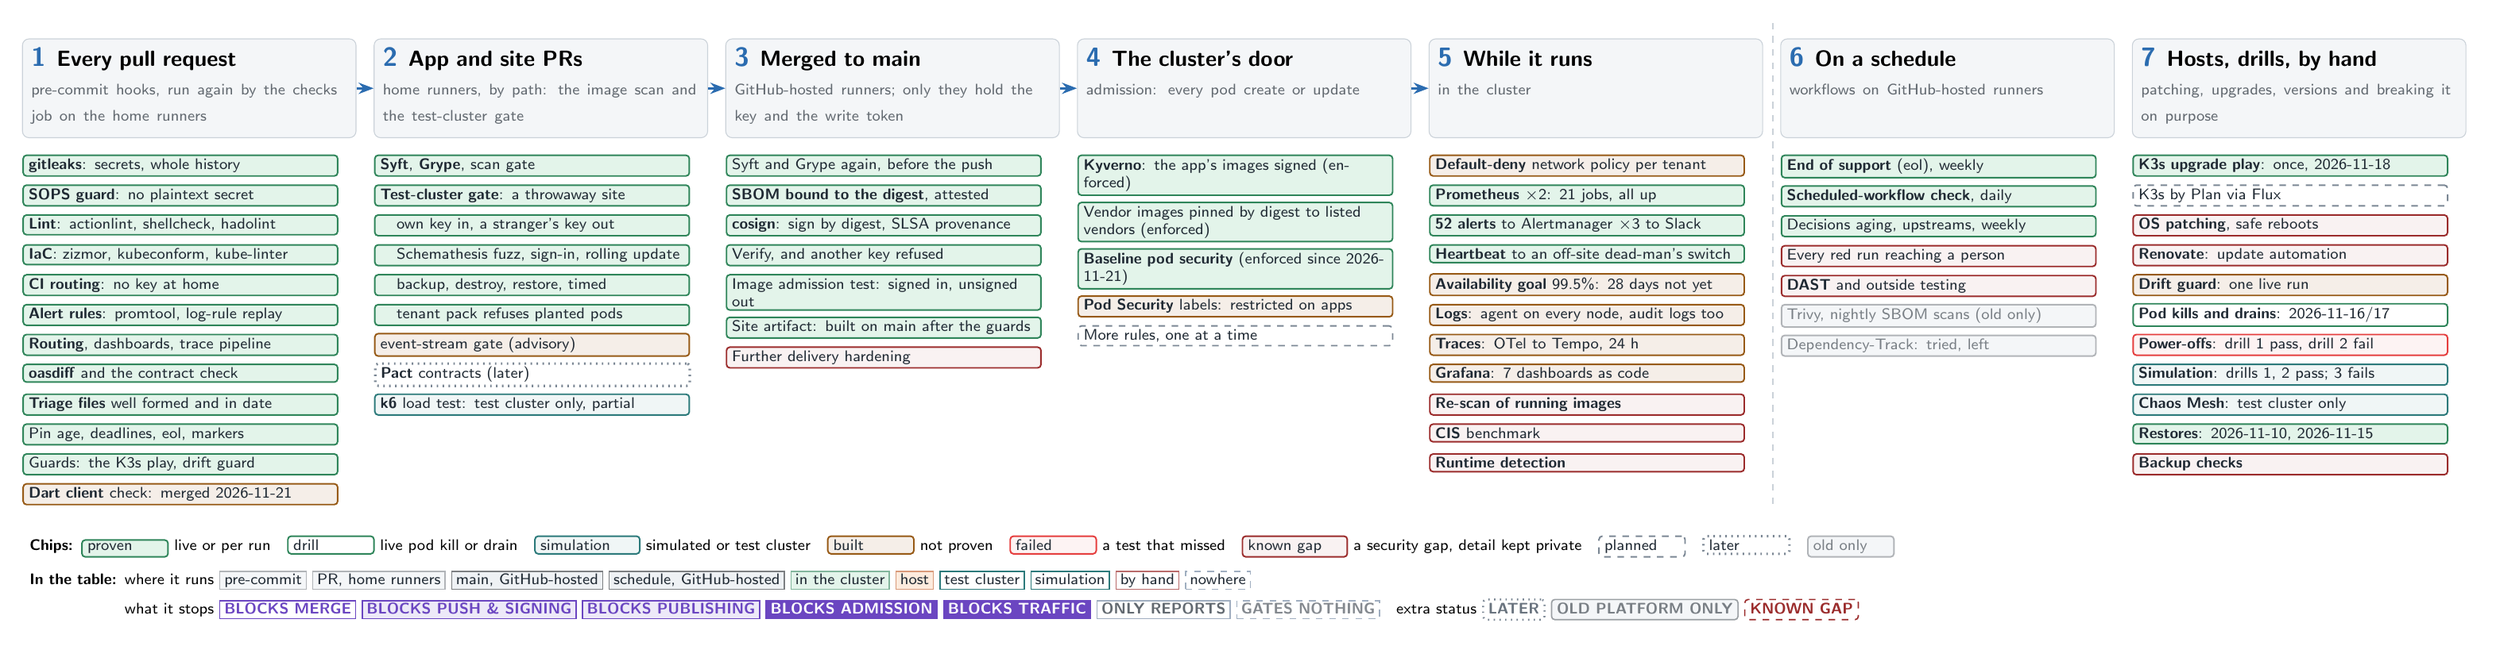
\begin{tikzpicture}[x=1cm, y=1cm,
  chip/.style={rounded corners=1.5pt, inner xsep=2.5pt, inner ysep=1.6pt, font=\scriptsize, line width=0.7pt,
    text width=4.85cm, align=left, text=ink},
  cP/.style={chip, draw=multi, fill=multifill},
  cD/.style={chip, draw=multi, fill=white},
  cS/.style={chip, draw=simc, fill=simc!7},
  cB/.style={chip, draw=builtc, fill=builtc!10},
  cPl/.style={chip, draw=plan, dashed, fill=white},
  cL/.style={chip, draw=plan, dotted, line width=1.1pt, fill=white},
  cO/.style={chip, draw=ink!35, fill=band, text=ink!60},
  cF/.style={chip, draw=failc, fill=failc!6},
  cX/.style={chip, draw=hand, fill=hand!6},
  cPR/.style={chip, draw=push, fill=white},
  hd/.style={draw=bandline, fill=band, rounded corners=3pt, text width=5.05cm, minimum height=1.55cm, align=left,
    inner sep=4pt, anchor=north west},
  col/.style={anchor=north west, text width=5.3cm, align=left, inner sep=0pt},
  stp/.style={-{Stealth[length=2.4mm]}, line width=1pt, draw=pull},
]
\newcommand{\C}[2]{\tikz[baseline=(c.base)]\node(c)[#1]{#2};\\[1.6pt]}
\newcommand{\Hd}[4]{\node[hd] (h#1) at (#2,0) {\parbox[t][1.3cm][t]{5.05cm}{\raggedright{\color{pull}\bfseries\large #1}\enspace{\bfseries\normalsize #3}\\[1pt]{\scriptsize\color{ink!70}#4}}};}
\Hd{1}{0}{Every pull request}{pre-commit hooks, run again by the checks job on the home runners}
\Hd{2}{5.62}{App and site PRs}{home runners, by path: the image scan and the test-cluster gate}
\Hd{3}{11.24}{Merged to main}{GitHub-hosted runners; only they hold the key and the write token}
\Hd{4}{16.86}{The cluster's door}{admission: every pod create or update}
\Hd{5}{22.48}{While it runs}{in the cluster}
\Hd{6}{28.10}{On a schedule}{workflows on GitHub-hosted runners}
\Hd{7}{33.72}{Hosts, drills, by hand}{patching, upgrades, versions and breaking it on purpose}
\foreach \a/\b in {1/2,2/3,3/4,4/5}{\draw[stp] (h\a.east) -- (h\b.west);}
\node[col] at (0,-1.85) {%
  \C{cP}{\textbf{gitleaks}: secrets, whole history}
  \C{cP}{\textbf{SOPS guard}: no plaintext secret}
  \C{cP}{\textbf{Lint}: actionlint, shellcheck, hadolint}
  \C{cP}{\textbf{IaC}: zizmor, kubeconform, kube-linter}
  \C{cP}{\textbf{CI routing}: no key at home}
  \C{cP}{\textbf{Alert rules}: promtool, log-rule replay}
  \C{cP}{\textbf{Routing}, dashboards, trace pipeline}
  \C{cP}{\textbf{oasdiff} and the contract check}
  \C{cP}{\textbf{Triage files} well formed and in date}
  \C{cP}{Pin age, deadlines, eol, markers}
  \C{cP}{Guards: the K3s play, drift guard}
  \C{cB}{\textbf{Dart client} check: merged 2026-11-21}};
\node[col] at (5.62,-1.85) {%
  \C{cP}{\textbf{Syft}, \textbf{Grype}, scan gate}
  \C{cP}{\textbf{Test-cluster gate}: a throwaway site}
  \C{cP}{\quad own key in, a stranger's key out}
  \C{cP}{\quad Schemathesis fuzz, sign-in, rolling update}
  \C{cP}{\quad backup, destroy, restore, timed}
  \C{cP}{\quad tenant pack refuses planted pods}
  \C{cB}{event-stream gate (advisory)}
  \C{cL}{\textbf{Pact} contracts (later)}
  \C{cS}{\textbf{k6} load test: test cluster only, partial}};
\node[col] at (11.24,-1.85) {%
  \C{cP}{Syft and Grype again, before the push}
  \C{cP}{\textbf{SBOM bound to the digest}, attested}
  \C{cP}{\textbf{cosign}: sign by digest, SLSA provenance}
  \C{cP}{Verify, and another key refused}
  \C{cP}{Image admission test: signed in, unsigned out}
  \C{cP}{Site artifact: built on main after the guards}
  \C{cX}{Further delivery hardening}};
\node[col] at (16.86,-1.85) {%
  \C{cP}{\textbf{Kyverno}: the app's images signed (enforced)}
  \C{cP}{Vendor images pinned by digest to listed vendors (enforced)}
  \C{cP}{\textbf{Baseline pod security} (enforced since 2026-11-21)}
  \C{cB}{\textbf{Pod Security} labels: restricted on apps}
  \C{cPl}{More rules, one at a time}};
\node[col] at (22.48,-1.85) {%
  \C{cB}{\textbf{Default-deny} network policy per tenant}
  \C{cP}{\textbf{Prometheus} \X2: 21 jobs, all up}
  \C{cP}{\textbf{52 alerts} to Alertmanager \X3 to Slack}
  \C{cP}{\textbf{Heartbeat} to an off-site dead-man's switch}
  \C{cB}{\textbf{Availability goal} 99.5\%: 28 days not yet}
  \C{cB}{\textbf{Logs}: agent on every node, audit logs too}
  \C{cB}{\textbf{Traces}: OTel to Tempo, 24 h}
  \C{cB}{\textbf{Grafana}: 7 dashboards as code}
  \C{cX}{\textbf{Re-scan of running images}}
  \C{cX}{\textbf{CIS} benchmark}
  \C{cX}{\textbf{Runtime detection}}};
\node[col] at (28.10,-1.85) {%
  \C{cP}{\textbf{End of support} (eol), weekly}
  \C{cP}{\textbf{Scheduled-workflow check}, daily}
  \C{cP}{Decisions aging, upstreams, weekly}
  \C{cX}{Every red run reaching a person}
  \C{cX}{\textbf{DAST} and outside testing}
  \C{cO}{Trivy, nightly SBOM scans (old only)}
  \C{cO}{Dependency-Track: tried, left}};
\node[col] at (33.72,-1.85) {%
  \C{cP}{\textbf{K3s upgrade play}: once, 2026-11-18}
  \C{cPl}{K3s by Plan via Flux}
  \C{cX}{\textbf{OS patching}, safe reboots}
  \C{cX}{\textbf{Renovate}: update automation}
  \C{cB}{\textbf{Drift guard}: one live run}
  \C{cD}{\textbf{Pod kills and drains}: 2026-11-16/17}
  \C{cF}{\textbf{Power-offs}: drill 1 pass, drill 2 fail}
  \C{cS}{\textbf{Simulation}: drills 1, 2 pass; 3 fails}
  \C{cS}{\textbf{Chaos Mesh}: test cluster only}
  \C{cP}{\textbf{Restores}: 2026-11-10, 2026-11-15}
  \C{cX}{\textbf{Backup checks}}};
\coordinate (cb) at (current bounding box.south);
\draw[bandline, line width=0.8pt, dashed] (27.98,0.25) -- (27.98,0 |- cb);
% key
\node[anchor=north west, font=\scriptsize, text width=39cm, align=left] at ($(0,0 |- cb)+(0,-0.35)$) {%
  \textbf{Chips:}\enspace
  \tikz[baseline=(k.base)]\node(k)[cP,text width=1.2cm]{proven};\ live or per run\quad
  \tikz[baseline=(k.base)]\node(k)[cD,text width=1.2cm]{drill};\ live pod kill or drain\quad
  \tikz[baseline=(k.base)]\node(k)[cS,text width=1.5cm]{simulation};\ simulated or test cluster\quad
  \tikz[baseline=(k.base)]\node(k)[cB,text width=1.2cm]{built};\ not proven\quad
  \tikz[baseline=(k.base)]\node(k)[cF,text width=1.2cm]{failed};\ a test that missed\quad
  \tikz[baseline=(k.base)]\node(k)[cX,text width=1.5cm]{known gap};\ a security gap, detail kept private\quad
  \tikz[baseline=(k.base)]\node(k)[cPl,text width=1.2cm]{planned};\quad
  \tikz[baseline=(k.base)]\node(k)[cL,text width=1.2cm]{later};\quad
  \tikz[baseline=(k.base)]\node(k)[cO,text width=1.2cm]{old only};\\[5pt]
  \textbf{In the table:}\enspace where it runs \wPC\ \wPR\ \wMain\ \wSched\ \wCl\ \wHost\ \wKind\ \wSim\ \wHand\ \wNone\quad
\\[3pt]\phantom{\textbf{In the table:}}\enspace what it stops \gMerge\ \gPush\ \gPub\ \gAdm\ \gTraffic\ \gRep\ \gNone\quad
  extra status \stLater\ \stOld\ \stGap};
\end{tikzpicture}
\end{center}
\vspace{-5mm}
{\footnotesize\renewcommand{\arraystretch}{1.06}
\begin{longtable}{@{}L{4.3cm}L{9.0cm}L{4.4cm}L{4.1cm}L{8.5cm}L{7.3cm}@{}}
\textbf{Tool or practice} & \textbf{What it does} & \textbf{Where it runs} & \textbf{What it stops} & \textbf{Status and evidence} & \textbf{What is open}\\\hline
\endfirsthead
\textbf{Tool or practice} & \textbf{What it does} & \textbf{Where it runs} & \textbf{What it stops} & \textbf{Status and evidence} & \textbf{What is open}\\\hline
\endhead
\Group{6}{Secrets, code and configuration: every pull request}
\textbf{gitleaks} & Pattern scan for secrets: the staged files on every commit, the whole git history in CI. & \wPC\ \wPR & \gMerge &
\stProven[2026-11-21] no leaks in the whole history. & Feature-frozen upstream; no replacement picked yet.\\
\textbf{SOPS plaintext guard} & Refuses any plaintext value in a site's secrets folder at any indent (the self-test plants 12 plaintext shapes and checks 17 cases). Secret-freshness and expiry hooks run beside it. & \wPC\ \wPR\ \wMain\ before the site artifact & \gMerge\ \gPub &
\stProven[2026-11-21]; an indentation blind spot found and fixed (2026-11-11). & \stGap\ key and token hygiene.\\
\textbf{Lint} & actionlint, shellcheck and hadolint over every workflow, script and Dockerfile, from images pinned by digest; a self-test proves each can fail. & \wPC\ \wPR & \gMerge & \stProven[2026-11-21]. & None stated.\\
\textbf{IaC scans} & zizmor (workflows: injection, unpinned actions), kubeconform (schemas), kube-linter (limits, root, host mounts, latest tags). A finding must be accepted in a triage file, and the acceptance expires. & \wPC\ \wPR & \gMerge &
\stProven[2026-11-21] every object valid; four planted faults found. & Coverage being widened.\\
\textbf{CI routing} & Fails if a job with a key, a write token or an environment runs on a home runner, or a pull request uses an Actions cache. & \wPC\ \wPR & \gMerge & \stProven[2026-11-21] passes in the checks job. & None stated.\\
\textbf{Other repository checks} & Balance across nodes, every manifest applied by something, documents match the live figures, endpoints, the runner host list, rollout scope, the image-pin age (a site's app digest at most 48 h behind its source). & \wPC\ \wPR & \gMerge\ (the minutes counter only prints) & \stProven[2026-11-21] checks job green. & \stGap\ coverage being widened.\\
\Group{6}{Contracts, the test-cluster gate and load}
\textbf{oasdiff} & Breaking-change gate on warn's API contract against main: a removed operation or property, a narrowed type, a new required parameter fail. & \wPC\ \wPR & \gMerge & \stProven[2026-11-21] the self-test plants four faults. & Sees only what the contract file shows.\\
\textbf{Contract check, Schemathesis} & Every app has a contract and every operation says who may call it; the test-cluster gate fuzzes the live warn app against its contract. & \wPC; \wKind\ in the gate & \gMerge & \stProven[2026-11-21]. & None stated.\\
\textbf{Generated Dart client check} & Fails when the contract, the generator or its options changed without a regeneration, or a generated file was edited by hand. & \wPC\ \wPR & \gMerge & \stBuilt\ merged 2026-11-21. & Its first red on a real contract change.\\
\textbf{Pact} & Consumer-driven contracts with a broker, designed on paper. & \wNone & -- & \stLater\ ``oasdiff now, Pact later''; never built on the old platform either. & Its trigger: a client released apart from the platform's repository.\\
\textbf{Test-cluster gate} & A throwaway kind site from the pull request: hand edits reverted, planted pods refused, own key admitted and a stranger's refused; sign-in, a trace with its SQL, the fuzz, a rolling update losing no request; backup, destroy, restore, timed. & \wPR\ (two of the CI hosts; median 36.8 min) & \gMerge & \stProven[2026-11-21]. & The event-stream gate stays advisory; the test cluster has no ingress, so the public path is not covered.\\
\textbf{k6 load test} & Thresholds in git; a compare script checks p95, p99 and errors against a baseline. & \wKind\ \wHand; the compare self-test \wPR & self-test \gMerge; the load test \gNone & \stSim[2026-11-11] partial record.\ \stPlanned\ against warn at home. & Waits on the 28-day retention.\\
\Group{6}{The image supply chain (the app's own image, warn)}
\textbf{Syft (SBOM)} & A CycloneDX SBOM of the warn image (Syft pinned by digest); an empty or wrong-format SBOM fails. & \wPR\ warn job; \wMain\ before the push & \gMerge\ \gPush & \stProven[2026-11-20] 278 packages. & \stGap\ supply-chain coverage being widened.\\
\textbf{Grype and the scan gate} & Matches the SBOM; the gate fails on a fixed High or Critical not accepted in triage. The self-test plants an old Alpine and a vulnerable log4j, and both must be refused. & \wPR\ \wMain & \gMerge\ \gPush\ (a blocked image is never signed) & \stProven[2026-11-20] both planted faults refused. & None stated.\\
\textbf{Image triage file} & Accepted findings in git: id, image, reason, an expiry within 90 days. The hook fails on a malformed or expired entry. & \wPC\ \wPR; read by the scans & \gMerge & \stProven[2026-11-21]. & Entries expire and must be re-read.\\
\textbf{SBOM binding and attestation} & Shows the SBOM's packages sit in the layers of the image the registry holds at that digest; cosign then attests the SBOM beside the signature. & \wMain & \gPush\ (main fails, nothing signed) & \stProven[2026-11-20] 278 packages in 4 of the image's 8 layers. & An SBOM store and a nightly re-match (planned).\\
\textbf{cosign signing and provenance} & Signs the warn image by digest with the key only main can use; attests SLSA provenance and the SBOM; a verify step checks it, and another key must be refused. & \wMain & \gPush\ (an empty key or a failed verify fails main) &
\stProven[2026-11-20]; green on every warn change since 2026-11-12. & Only the app's own images are signed; vendor images are pinned by digest.\\
\textbf{Site artifact (publish)} & Builds the Flux OCI artifact from main, after the render and plaintext guards. & \wMain & \gPub\ on the guards & \stProven\ on every merge. & \stGap\ further delivery hardening.\\
\textbf{Trivy} & Old platform: a nightly host-scan DaemonSet and SBOM CronJobs. In the new platform it lost a spike to Syft and Grype; its release tags were hijacked in March 2026. & \wNone\ in V2.0 & -- & \stOld & Its jobs moved to build time; a host-scan successor is planned.\\
\textbf{Dependency-Track} & Old platform: SBOMs re-derived nightly and re-analysed daily. Tried in the new platform: a 2.3 GB JVM, 24 Highs nobody could act on, and it missed the real one. & \wNone\ in V2.0 & -- & \stOld\ the trial's verdict was ``leave''. & Its job: Syft, Grype and the triage file at build time; the re-check of running images below. Findings triage stays open.\\
\textbf{Scan of running images} & Lists every pod's image digest, then Syft, Grype and the triage gate; fails on a short list, a missed canary or an unscanned image (it raises an alert). Planned: weekly, then a nightly re-match of stored SBOMs once an SBOM store exists. & \wCl\ (a CronJob) & \gRep\ (the alert) &
\stBuilt\ self-test and a test-cluster run (2026-11-11); being switched on. & \stGap\\
\Group{6}{The cluster's door and walls}
\textbf{Kyverno: signed app images} & The app's images must be signed by the CI key. Two replicas. & \wCl; also \wKind\ and an admission test on \wMain & \gAdm\ (enforced, fails closed) &
\stProven[2026-11-20] signed admitted, unsigned refused over 72 rounds. & Admission with GHCR unreachable never tried.\\
\textbf{Kyverno: pinned vendor images} & A vendor image must come from a listed repository and be pinned by digest. & \wCl & \gAdm & \stProven[2026-11-20] an untagged image refused, the pinned one admitted. & None stated.\\
\textbf{Kyverno: baseline pod security} & Refuses host namespaces, privileged pods, host paths, added capabilities, host ports, seccomp, AppArmor and SELinux changes, proc mount, sysctls, with named exceptions for the node agents. & \wCl & \gAdm\ since 2026-11-21 &
\stProven[2026-11-21] probe: 4 refusals, 2 admissions; 113 reports pass. & More rules are added one at a time.\\
\textbf{Pod Security Admission} & Namespace labels: restricted for the tenant pack and the apps; a few node agents need host access under named exceptions. & \wCl\ (built into K3s) & \gAdm & \stBuilt\ labels read live.\ \stSim\ the test cluster refuses five planted pods. & \stGap\\
\textbf{Network policies} & Default-deny in and out in the tenant pack, plus named allows (kube-router). & \wCl & \gTraffic & \stBuilt\ steady state holds (home probe 2026-11-10).\ \stSim\ test cluster. & \stGap\\
\textbf{CIS benchmark} & kube-bench with the K3s profile, pinned by digest: the node and K3s settings against the benchmark. & \wCl & \gRep & \stGap\ benchmarks are being worked on. & --\\
\textbf{Runtime detection} (Falco) & Watching running workloads for threats. & -- & -- & \stGap\ being worked on. & --\\
\textbf{DAST: ZAP, Nuclei, an outside tester} & ZAP baseline and Nuclei against the public entrance on a schedule, the report in git, a planted weakness always found; a quarterly outside tester. & -- & -- & \stGap\ outside testing is being worked on; the public entrance opens only after it meets the platform's bar. & --\\
\Group{6}{Seeing it: metrics, alerts, logs, traces and scheduled checks}
\textbf{Prometheus and exporters} & Prometheus \X2 scrapes 21 jobs every 30 s (7 days); kube-state-metrics, the node exporter on six nodes, blackbox probes, a DNS probe on every node. & \wCl & \gRep & \stProven[2026-11-21] all 21 jobs up.\ \stSim[2026-11-18] test-cluster HA trial. & Backup and node faults, a 14-day window. A monitoring gap after the K3s upgrade was caught by no gate.\\
\textbf{Alert rules and their tests} & 52 alerts and 16 recording rules, 179 promtool cases; 5 log alerts in Loki; a hook checks every series a rule reads exists. & rules \wCl; tests \wPC\ \wPR & \gMerge\ on a failing test & \stSim[2026-11-11] faults fired on a scratch test cluster; rules loaded live; tests green on every PR. & More alert families; runbook links unchecked; no disk-fill forecast.\\
\textbf{Alert delivery: Slack and an off-site heartbeat} & Alertmanager \X3: critical to Slack at once (repeat 1 h), warning (12 h). A heartbeat every minute to an off-site dead-man's switch that tells the owner by Slack and e-mail. A hook proves the routing. & \wCl; the heartbeat service off-site & routing hook \gMerge; delivery \gRep &
\stProven[2026-11-16] a test critical in Slack, and a silent house reported by the heartbeat. 120 sent to Slack, 0 failed (2026-11-21). & Paging is deliberately simple. \stGap\ every failure reaching a person. A real outage (router unplugged) never tried.\\
\textbf{Availability goal} & 99.5\% over 28 days: blackbox probes, success-ratio and budget rules, burn-rate alerts (critical above 14.4, warning above 6). & \wCl & \gRep & \stBuilt\ live since 2026-11-17, tested on every PR. 28 days of data cannot exist with 7-day retention; the sign-in probe missed a login-database outage. & Retention, a database-aware probe.\\
\textbf{Logs} & An OpenTelemetry log agent on every node collects container and audit logs into Loki; a replay hook proves rules fire on real lines. & \wCl; replay \wPR & hook \gMerge; runtime \gRep & \stBuilt\ logs from every node (2026-11-15).\ \stSim[2026-11-19] Loki outage: no line lost. & Keeping logs in more than one copy (planned); a live log-alert test.\\
\textbf{Traces} & The OTel gateway collector to Tempo (24 h); dropped-span alerts; a hook reads a span back by id, also after a Tempo restart. & \wCl; hook \wPR & \gMerge\ (hook, test-cluster gate) & \stBuilt\ live; the trace-to-log link and a live restart are not recorded. & Tempo's memory; the AI host's way in.\\
\textbf{Dashboards} & 7 Grafana dashboards as code; a hook checks titles, units, the data source and the wiring. & \wCl; hook \wPR & \gMerge & \stBuilt\ live; Grafana's own state is not persisted. & Grafana persistence.\\
\textbf{Runner liveness alert} & A script on the backup host, every 2 minutes, probes each runner host and posts to Alertmanager. & \wHost; self-tests \wPR & \gRep & \stBuilt\ proven 2026-11-10 against the old cluster only. & \stGap\ every failure reaching a person.\\
\textbf{Scheduled-workflow check} & Fails when a scheduled workflow's last run failed or its schedule stopped or never fired; a known red is muted until a date. & \wSched\ daily & \gRep & \stProven[2026-11-21]. & \stGap\ every red run reaching a person.\\
\textbf{Deadlines and end of support} & Deadlines inside their lead time; eight products against endoflife.date with 60 days' lead; proposed design records older than 14 days; archived or silent upstreams. & hooks \wPR; schedules \wSched\ weekly & hooks \gMerge; schedules \gRep &
\stProven[2026-11-16] went red on the admission controller's old minor and green after the upgrade. & \stGap\ every red run reaching a person.\\
\textbf{Drift guard} & Reads the live cluster: live-only objects, Flux orphans, Helm releases off their pinned chart, stale allow-list entries; can raise an alert. & self-test \wPR; the live run \wHand & hooks \gMerge; the live run \gNone & \stBuilt\ one live run, no drift (2026-11-14). & \stGap\\
\Group{6}{Keeping current: patching, upgrades and versions}
\textbf{OS patching} & Old platform: security updates installed daily, the reboot flag written and patch age measured. The new host baseline requires the same, for every host. & \wHost & -- & \stGap\ keeping hosts current is being worked on.\ \stOld\ as a measured job. & --\\
\textbf{kured} & Safe reboots after kernel updates: one node at a time, storage healthy first, an alert if it stops acting. & -- & -- & \stGap\ being worked on.\ \stOld & The settings that cost the old platform a month are written down.\\
\textbf{K3s upgrades} & An Ansible play: one minor at a time, an etcd snapshot first, unforced drains, a health gate between nodes; the target is given by hand, so no merge starts one. The end-of-support check warns 60 days ahead. & \wHost\ \wHand\ from the operator seat; the guard hook \wPR & hook \gMerge; the play refuses on a failed gate &
\stProven[2026-11-18] six nodes moved one minor in 11.5 min (then one gap no gate caught). & By Plan through Flux (proposed); the play's check mode times out.\\
\textbf{Renovate} & Reads version markers in the repository (charts, digests, scanners); a 3-day cooldown, 14 days and no automerge for security tools; a hook checks every marker is read. & config in the repository; hook \wPR & hook \gMerge; Renovate only proposes &
\stBuilt\ configured.\ \stGap\ update automation is being worked on. & Operators, Flux and automerge rules.\\
\Group{6}{Breaking it on purpose: drills, chaos, backups and restores}
\textbf{Pod-kill and failover drills} & Pod deletes, drains and switchovers on the live site under probes: warn, Keycloak, Traefik, CoreDNS, Kyverno, poolers, primaries, standbys, the operator and the plugin. & \wHand\ on the live site & \gNone\ (evidence) & \stDrill[2026-11-16/17] 17 records, 15 pass; the warn primary kill failed (48.6 s) and passed again after the pooler fix;\ \stFailed\ both plugin pods, 35.2 s against 30 s. & The plugin's extra seconds; the 27.9 s margin.\\
\textbf{Power-off drills} & The owner powers off a real node by a run sheet; a probe measures. & \wHand\ on the live site & \gNone; a live drill only after it passes in simulation & \stProven[2026-11-19] drill 1.\ \stFailed[2026-11-19] drill 2 (the old DNS design). & Restart from drill 1 after the DNS change; drills 4--7.\\
\textbf{Simulations} & A home-shaped simulated cluster (k3d: 3 servers, 3 agents, on the operator seat) rehearses each power-off drill first; the drill-3 figures come from it. & \wSim\ on the operator seat; not in CI & \gNone & \stSim[2026-11-20] drills 1 and 2 pass.\ \stFailed[in simulation] drill 3. & Drills 4--7 and a nightly simulation are not built.\\
\textbf{Chaos Mesh} & Fault injection, picked after a test-cluster spike: a script installs it and runs experiments. & \wKind\ \wHand; nothing on the live site & \gNone & \stSim\ the spike only.\ \stPlanned\ scheduled injection with a kill switch. The old platform ran two schedules. & The owner approves a schedule.\\
\textbf{Backups} & Nightly base backups (warn, Keycloak) and WAL to Garage, outside the cluster; alerts when a backup is too old or missing. Second copy: the NAS pulls with a read-only key; an off-site copy follows. & \wCl\ \wHost & \gRep &
\stBuilt\ copies 1 and 2; no restore from the NAS yet.\ \stGap\ backup checks and the schedule of the extra copies. & The off-site copy; a restore from each copy.\\
\textbf{Restore drills} & A backup, destroy and restore in every test-cluster gate, timed; live restores from Garage by hand. & \wKind\ in \wPR; live \wHand & test cluster \gMerge & \stProven[2026-11-10] warn.\ \stProven[2026-11-15] login, 13 MB in 81 s. & No scheduled restore drill; point-in-time, total-loss and off-site restores.\\
\end{longtable}}

% ================================================================== 8. NOT PROVEN YET
\Part{8}{What is not proven yet}{The top open items from sections 4 to 7, ordered by risk: first what can lose data or keys for good, then what stops the apps, then what blinds us.
The order is this booklet's reading, not an owner decision. Security gaps are counted here but described only in general.}
{\small
\begin{longtable}{@{}r L{7.0cm} L{14.6cm} L{11.2cm} L{4.8cm}@{}}
\textbf{\#} & \textbf{Item} & \textbf{Why it is a risk} & \textbf{What would close it} & \textbf{Status}\\\hline
\endhead
\Group{5}{Can lose data or keys for good}
1 & Key custody & A key that cannot be restored is an unproven recovery. & Key custody and a recovery test. & \stGap\\
2 & etcd snapshots stay on the servers; no scheduled off-node copy & Two servers lost means a reset from the third's last snapshot. The reset was never run. & An off-node copy on a schedule, the schedule written in git (the owner's go); a timed restore on a scratch cluster. & \stOpen\\
3 & Backup copies and checks & Backups go to stores outside the cluster, with more copies, including off-site, being built; backup checks and the schedule of the extra copies are known gaps being worked on. The window to stopped writes when archiving stops is unmeasured. & The extra copies on a schedule, a restore from each, backup checks; drill 7. & \stGap\\
4 & No off-site, point-in-time or total-loss restore & Three restores passed: two from copy 1 into a scratch cluster (warn about 60 s, a few MB; login 13 MB in 81 s) and one on the old platform from its NAS copy (2026-11-08). None was off-site, point-in-time or a total loss. & Restore drills with recorded recovery times. & \stPlanned\\
5 & Logs and traces in more than one copy & Logs, including audit logs, are collected from every node; keeping them in more than one copy is planned. The rule and its fix are only proposed. & Agree the proposal; a design record for Garage across machines or Ceph. & \stProp\\
\Group{5}{Can stop the apps}
6 & Drill 3: a node with a Traefik and a pooler replica & In simulation about half of new connections failed for about 45 s, a few more up to 90 s, against targets of 30 s and 10 s. & The owner picks a fix (or new targets), it passes in simulation, then the live drill 3. & \stFailed[in simulation]\\
7 & Delivery and admission hardening & Known gaps in how a change is trusted on its way to the cluster are being worked on. & The planned steps, each proven by a test that can fail. & \stGap\\
8 & Server power-offs (drills 4, 5, 6) & A server may hold the API address, the ingress address, the operator and plugin leaders or a primary; none of these moves has been simulated or run live. & Simulations of drills 4--7, then live. & \stNotProven\\
9 & Backup plugin with both pods down & Failover missed its target (35 s against 30 s); the target itself is an owner question (30 s or 60 s). & The extra seconds fixed; the owner's target; drill 4. & \stFailed[2026-11-17]\\
10 & Drill 2 after the DNS change; drill 1 again & Drill 2 failed live on the old design; the fix passed only in simulation. Zero of 27 rows are fixed. & Live drills 1 and 2 again. & \stSim[2026-11-20]\\
11 & Kyverno both down, and GHCR down & With both replicas down no pod starts where its rules apply (Kyverno itself can still restart); whether a warn pod is admitted with GHCR unreachable was never tried. & A both-down test; an offline admission test; a registry mirror. & \stNotProven\\
12 & Flux single replica & No change, fix or containment lands while it is down. & Two replicas with a spread, or the owner accepts one. & \stOpen\\
13 & A whole-house power cut & Never run on real machines. No scripted shutdown, no wake-on-LAN; what the laptop batteries do is not analysed. & A scripted shutdown and start, after the runbooks are run by a cold reader. & \stPlanned\\
\Group{5}{Can blind us or slow recovery}
14 & House DNS: open or accepted? & The register says open, the run sheet says accepted. It was never stopped to see what breaks. & The owner's answer; a second resolver; the public name takes it off the core path. & \stOpen\\
15 & The operator seat, GitHub access and the backup and AI host have no register row & Administration, every merge, and backup copy 1. & Register rows; protecting the accounts that can merge (a known gap); the host held to the bar. & \stOpen\\
16 & One person & Every drill and every key need the owner at the machines. & A second responder; a cold-reader runbook run. & \stPlanned\\
17 & Owner questions & The entry-node wording; which server holds the etcd leader; Slack on the phone as a phone path. & The owner's answers, written into the register. & \stOpen\\
18 & Rook-Ceph & Wanted for learning and for a second stateful app. No design record and no plan item yet. & A design record first, then a plan item. & \stWanted\\
\Group{5}{Can leave a known weakness in place or unseen (the safety net, section 7)}
19 & Keeping current, and watching & Keeping hosts and images current, watching for threats at runtime, and making every failure reach a person are known gaps being worked on (patching, update automation, re-scans, benchmarks, runtime and outside testing, alert delivery). & The planned steps, each proven by a test that can fail. & \stGap\\
\end{longtable}}

\end{document}
